\documentclass[11pt,a4paper,twoside,openany]{book}
\usepackage[a4paper,left=28mm,right=28mm,top=28mm,bottom=26mm,headsep=8mm]{geometry}
\usepackage[T1]{fontenc}
\usepackage{mathptmx}
\usepackage[letterspace=120]{microtype}
\usepackage{amsmath,amssymb,amsthm,bm}
\usepackage{graphicx}
\usepackage{booktabs,array,longtable}
\usepackage{colortbl}
\usepackage{xcolor}
\definecolor{dgblue}{HTML}{1B3A5C}
\definecolor{dghead}{HTML}{EDF0F4}
\definecolor{dgpale}{HTML}{F3F5F8}
\usepackage[font={small},labelfont={bf,color=dgblue},labelsep=space,justification=justified,singlelinecheck=false,figurename=Figure,skip=5pt]{caption}
\captionsetup[table]{position=top}
\usepackage{titlesec,titletoc}
\usepackage{enumitem}
\usepackage{fancyhdr}
\usepackage{placeins}
\usepackage{needspace}
\usepackage[most]{tcolorbox}
\usepackage{cite}
\usepackage[colorlinks=true,allcolors=dgblue]{hyperref}
\usepackage{xurl}
\urlstyle{same}
\arrayrulecolor{dgblue}
\setlength{\heavyrulewidth}{0.9pt}\setlength{\lightrulewidth}{0.45pt}
\setlength{\aboverulesep}{0pt}\setlength{\belowrulesep}{0pt}
\renewcommand{\arraystretch}{1.22}
\newcommand{\NumBaseGapMin}{0.27}
\newcommand{\NumBaseGapMax}{0.40}
\newcommand{\NumBaseGainMin}{0.00}
\newcommand{\NumBaseGainMax}{0.02}
\newcommand{\NumBaseSensMin}{0.00}
\newcommand{\NumBaseSensMax}{0.02}
\newcommand{\NumBaseSampMin}{-0.01}
\newcommand{\NumBaseSampMax}{0.00}
\newcommand{\NumBaseGainSig}{10}
\newcommand{\NumBaseSampNull}{11}
\newcommand{\NumBaseHzA}{83}
\newcommand{\NumBaseHzB}{113}
\newcommand{\NumBaseFiveSig}{12}
\newcommand{\NumBaseMaxSig}{12}
\newcommand{\NumBaseEceMMin}{0.03}
\newcommand{\NumBaseEceMMax}{0.07}
\newcommand{\NumBaseEceOMin}{0.04}
\newcommand{\NumBaseEceOMax}{0.13}
\newcommand{\NumBaseEcePMin}{0.34}
\newcommand{\NumBaseEcePMax}{0.43}
\newcommand{\NumLagGapMin}{0.27}
\newcommand{\NumLagGapMax}{0.40}
\newcommand{\NumLagGainMin}{0.01}
\newcommand{\NumLagGainMax}{0.04}
\newcommand{\NumLagSensMin}{0.00}
\newcommand{\NumLagSensMax}{0.01}
\newcommand{\NumLagSampMin}{-0.01}
\newcommand{\NumLagSampMax}{0.00}
\newcommand{\NumLagGainSig}{12}
\newcommand{\NumLagSampNull}{11}
\newcommand{\NumLagHzA}{83}
\newcommand{\NumLagHzB}{113}
\newcommand{\NumLagFiveSig}{11}
\newcommand{\NumLagMaxSig}{12}
\newcommand{\NumLagEceMMin}{0.01}
\newcommand{\NumLagEceMMax}{0.07}
\newcommand{\NumLagEceOMin}{0.05}
\newcommand{\NumLagEceOMax}{0.13}
\newcommand{\NumLagEcePMin}{0.34}
\newcommand{\NumLagEcePMax}{0.44}
\newcommand{\NumLowGapMin}{0.28}
\newcommand{\NumLowGapMax}{0.40}
\newcommand{\NumLowGainMin}{0.00}
\newcommand{\NumLowGainMax}{0.02}
\newcommand{\NumLowSensMin}{0.00}
\newcommand{\NumLowSensMax}{0.02}
\newcommand{\NumLowSampMin}{-0.01}
\newcommand{\NumLowSampMax}{0.01}
\newcommand{\NumLowGainSig}{8}
\newcommand{\NumLowSampNull}{10}
\newcommand{\NumLowHzA}{120}
\newcommand{\NumLowHzB}{154}
\newcommand{\NumLowFiveSig}{11}
\newcommand{\NumLowMaxSig}{12}
\newcommand{\NumLowEceMMin}{0.02}
\newcommand{\NumLowEceMMax}{0.11}
\newcommand{\NumLowEceOMin}{0.02}
\newcommand{\NumLowEceOMax}{0.14}
\newcommand{\NumLowEcePMin}{0.34}
\newcommand{\NumLowEcePMax}{0.44}
\newcommand{\NumCombGapMin}{0.28}
\newcommand{\NumCombGapMax}{0.40}
\newcommand{\NumCombGainMin}{0.00}
\newcommand{\NumCombGainMax}{0.02}
\newcommand{\NumCombSensMin}{0.00}
\newcommand{\NumCombSensMax}{0.01}
\newcommand{\NumCombSampMin}{-0.01}
\newcommand{\NumCombSampMax}{0.01}
\newcommand{\NumCombGainSig}{10}
\newcommand{\NumCombSampNull}{12}
\newcommand{\NumCombHzA}{201}
\newcommand{\NumCombHzB}{258}
\newcommand{\NumCombFiveSig}{11}
\newcommand{\NumCombMaxSig}{12}
\newcommand{\NumCombEceMMin}{0.02}
\newcommand{\NumCombEceMMax}{0.09}
\newcommand{\NumCombEceOMin}{0.02}
\newcommand{\NumCombEceOMax}{0.13}
\newcommand{\NumCombEcePMin}{0.34}
\newcommand{\NumCombEcePMax}{0.43}
\newcommand{\NumLisGapMin}{0.09}
\newcommand{\NumLisGapMax}{0.34}
\newcommand{\NumLisGainMin}{0.00}
\newcommand{\NumLisGainMax}{0.02}
\newcommand{\NumLisSensMin}{0.01}
\newcommand{\NumLisSensMax}{0.02}
\newcommand{\NumLisSampMin}{-0.01}
\newcommand{\NumLisSampMax}{0.01}
\newcommand{\NumLisGainSig}{8}
\newcommand{\NumLisSampNull}{12}
\newcommand{\NumLisHzA}{100}
\newcommand{\NumLisHzB}{202}
\newcommand{\NumLisFiveSig}{12}
\newcommand{\NumLisMaxSig}{12}
\newcommand{\NumLisEceMMin}{0.08}
\newcommand{\NumLisEceMMax}{0.41}
\newcommand{\NumLisEceOMin}{0.11}
\newcommand{\NumLisEceOMax}{0.44}
\newcommand{\NumLisEcePMin}{0.34}
\newcommand{\NumLisEcePMax}{0.45}
\newcommand{\NumLinConst}{90}
\newcommand{\NumLinExc}{53}
\newcommand{\NumLinErr}{-4}
\newcommand{\NumLinErrAbs}{4}
\newcommand{\NumCbN}{51}
\newcommand{\NumCbB}{0.0256}
\newcommand{\NumCbT}{-6.6}
\newcommand{\NumCbSd}{0.16}
\newcommand{\NumCbBias}{1.62}
\newcommand{\NumLisN}{46}
\newcommand{\NumLisHeld}{53}
\newcommand{\NumLisB}{0.0235}
\newcommand{\NumLisT}{-2.3}
\newcommand{\NumLisBLo}{0.0203}
\newcommand{\NumLisBHi}{0.0265}
\newcommand{\NumLisTLo}{-4.2}
\newcommand{\NumLisTHi}{-0.9}
\newcommand{\NumLisBiasHeld}{1.02}
\newcommand{\NumLisAccHeld}{1.37}
\newcommand{\NumLisAccFit}{1.33}
\newcommand{\NumLisGen}{32}
\newcommand{\NumLisRatio}{5.9}
\newcommand{\NumLisSd}{0.38}
\newcommand{\NumLisOrcAMin}{0.88}
\newcommand{\NumLisOrcAMax}{0.92}
\newcommand{\NumLisOrcBMin}{1.00}
\newcommand{\NumLisOrcBMax}{1.00}
\newcommand{\NumLisEceAMMin}{0.28}
\newcommand{\NumLisEceAMMax}{0.41}
\newcommand{\NumLisEceAPMin}{0.42}
\newcommand{\NumLisEceAPMax}{0.45}
\newcommand{\NumLisEceBMMin}{0.08}
\newcommand{\NumLisEceBMMax}{0.20}
\newcommand{\NumLisEceBPMin}{0.34}
\newcommand{\NumLisEceBPMax}{0.41}
\newcommand{\NumLisPrevMin}{0.08}
\newcommand{\NumLisPrevMax}{0.38}

\newcommand{\DatNFull}{373}
\newcommand{\DatNLis}{102}
\newcommand{\DatNSp}{51}
\newcommand{\TabAUC}{\begin{table*}[t]\centering\footnotesize
\caption{AUC of the five scores from a DS18B20 record sampled every 15\,min (baseline run, 4\,000 trips per row). The best score in each row is in bold. The last two columns give the same kinetic score with an ideal sensor sampled every minute, and the oracle that knows each trip's biology}\label{tab:auc}
\begin{tabular}{@{}lllccccccc@{}}\toprule\rowcolor{dghead}
Limit & Product & $cv$ & CSL & Degree-h $>4$\,\textdegree C & Time $>5$\,\textdegree C & Time $>8$\,\textdegree C & $T_{\max}$ & Ideal, 1 min & Oracle\\\midrule
A & Pouch & 0.00 & \textbf{0.705} & 0.690 & 0.635 & 0.569 & 0.629 & 0.718 & 1.000\\
A & Pouch & 0.10 & \textbf{0.651} & 0.634 & 0.599 & 0.557 & 0.591 & 0.659 & 1.000\\
A & Pouch & 0.25 & \textbf{0.620} & 0.619 & 0.591 & 0.561 & 0.602 & 0.627 & 1.000\\
A & Crate & 0.00 & \textbf{0.722} & 0.711 & 0.701 & 0.586 & 0.638 & 0.732 & 1.000\\
A & Crate & 0.10 & \textbf{0.674} & 0.666 & 0.657 & 0.577 & 0.611 & 0.687 & 1.000\\
A & Crate & 0.25 & \textbf{0.599} & 0.596 & 0.592 & 0.541 & 0.571 & 0.603 & 1.000\\
\midrule
B & Pouch & 0.00 & \textbf{0.710} & 0.686 & 0.636 & 0.564 & 0.587 & 0.723 & 1.000\\
B & Pouch & 0.10 & \textbf{0.656} & 0.634 & 0.606 & 0.539 & 0.564 & 0.670 & 1.000\\
B & Pouch & 0.25 & \textbf{0.604} & 0.594 & 0.565 & 0.531 & 0.549 & 0.608 & 1.000\\
B & Crate & 0.00 & \textbf{0.708} & 0.696 & 0.687 & 0.600 & 0.629 & 0.724 & 1.000\\
B & Crate & 0.10 & \textbf{0.676} & 0.670 & 0.663 & 0.585 & 0.611 & 0.686 & 1.000\\
B & Crate & 0.25 & \textbf{0.603} & 0.595 & 0.591 & 0.538 & 0.552 & 0.608 & 1.000\\
\bottomrule\end{tabular}\end{table*}}

\newcommand{\TabBudget}{\begin{table}[t]\centering\footnotesize
\caption{Loss budget: mean AUC over the 12 settings of each run as information is removed, and the range of the biology gap (oracle minus ideal sensor)}\label{tab:budget}
\setlength{\tabcolsep}{3.2pt}
\begin{tabular}{@{}lcccccc@{}}\toprule\rowcolor{dghead}
Run & Oracle & Ideal & PT1000 & DS18B20 & DS18B20 & Biology gap\\
 & & 1\,min & 15\,min & 15\,min & 60\,min & \\\midrule
Baseline & 1.000 & 0.671 & 0.670 & 0.661 & 0.662 & 0.27--0.40\\
Extra lag & 0.988 & 0.652 & 0.652 & 0.644 & 0.645 & 0.27--0.40\\
Low load & 1.000 & 0.667 & 0.666 & 0.656 & 0.657 & 0.28--0.40\\
Milk flora & 1.000 & 0.664 & 0.663 & 0.654 & 0.653 & 0.28--0.40\\
\textit{Listeria} & 0.950 & 0.738 & 0.737 & 0.725 & 0.726 & 0.09--0.34\\
\bottomrule\end{tabular}\end{table}}

\newcommand{\TabContrasts}{\begin{table*}[t]\centering\footnotesize
\caption{Paired AUC differences on identical trips: minimum/maximum over the 12 settings of each run, with the number of settings (of 12) whose 95\,\% paired-bootstrap interval excludes zero in brackets}\label{tab:contrasts}
\begin{tabular}{@{}lccccc@{}}\toprule\rowcolor{dghead}
Contrast & Baseline & Extra lag & Low load & Milk flora & \textit{Listeria}\\\midrule
CSL $-$ degree-h & 0.001/0.023 (10) & 0.006/0.037 (12) & 0.001/0.023 (8) & 0.004/0.025 (10) & 0.002/0.023 (8)\\
CSL $-$ time $>5$\,\textdegree C & 0.008/0.074 (12) & 0.001/0.104 (11) & 0.005/0.066 (11) & 0.006/0.075 (11) & 0.010/0.077 (12)\\
PT1000 $-$ DS18B20 & 0.003/0.015 (9) & 0.003/0.013 (7) & 0.005/0.018 (10) & 0.002/0.015 (8) & 0.005/0.020 (8)\\
60\,min $-$ 1\,min & -0.008/0.004 (1) & -0.008/0.004 (1) & -0.011/0.008 (2) & -0.009/0.006 (0) & -0.008/0.009 (0)\\
Adaptive $-$ 1\,min & -0.006/0.005 (0) & -0.006/0.006 (0) & -0.008/0.009 (1) & -0.007/0.006 (0) & -0.006/0.009 (0)\\
\bottomrule\end{tabular}\end{table*}}

\newcommand{\TabCal}{\begin{table*}[t]\centering\footnotesize
\caption{Calibration: range of expected calibration error over the 12 settings, and mean Brier score, for each run. Lower is better}\label{tab:cal}
\begin{tabular}{@{}lccccc@{}}\toprule\rowcolor{dghead}
Variant & Baseline & Extra lag & Low load & Milk flora & \textit{Listeria}\\\midrule
Probability, matched prior & 0.03--0.07 / 0.231 & 0.01--0.07 / 0.236 & 0.02--0.11 / 0.233 & 0.02--0.09 / 0.234 & 0.08--0.41 / 0.216\\
Probability, overconfident & 0.04--0.13 / 0.237 & 0.05--0.13 / 0.244 & 0.02--0.14 / 0.238 & 0.02--0.13 / 0.239 & 0.11--0.44 / 0.218\\
Single alarm & 0.33--0.43 / 0.380 & 0.34--0.44 / 0.391 & 0.34--0.44 / 0.386 & 0.34--0.43 / 0.385 & 0.34--0.45 / 0.400\\
\bottomrule\end{tabular}\end{table*}}

\newcommand{\TabDataComp}{\begin{table}[t]\centering\footnotesize
\caption{Composition of the compiled ComBase milk database by organism. $n$: records; Rate: maximum growth rate stated; Curve: growth curve only; None: no growth reported; N/T: rate not transcribed}\label{tab:dcomp}
\setlength{\tabcolsep}{3pt}
\begin{tabular}{@{}lccccc@{}}\toprule\rowcolor{dghead}
Organism & $n$ & Rate & Curve & None & N/T\\\midrule
\textit{L.~monocytogenes/innocua} & 149 & 102 & 43 & 0 & 4\\
\textit{Bacillus cereus} & 94 & 47 & 36 & 3 & 8\\
\textit{Escherichia coli} & 66 & 22 & 15 & 4 & 25\\
\textit{Salmonella} spp. & 25 & 4 & 7 & 13 & 1\\
Campylobacteraceae & 16 & 0 & 13 & 0 & 3\\
Shigellae & 11 & 0 & 10 & 0 & 1\\
\textit{Cronobacter} spp. & 6 & 0 & 5 & 0 & 1\\
Aerobic spoilage bacteria & 4 & 4 & 0 & 0 & 0\\
Lactic acid bacteria & 1 & 0 & 1 & 0 & 0\\
Other & 1 & 0 & 1 & 0 & 0\\
\midrule Total & 373 & 179 & 131 & 20 & 43\\
\bottomrule\end{tabular}\end{table}}

\graphicspath{{../paper/fig/}{fig/}}
% headings
\titleformat{\chapter}[display]{\normalfont\color{dgblue}}{\fontsize{13}{15}\selectfont\textls[200]{\MakeUppercase{\chaptertitlename}}~\thechapter}{6pt}{\fontsize{24}{29}\selectfont\bfseries}[\vspace{4pt}{\titlerule[1.2pt]}]
\titlespacing*{\chapter}{0pt}{10pt}{26pt}
\titleformat{\section}{\needspace{5\baselineskip}\normalfont\large\bfseries\color{dgblue}}{\thesection}{0.8em}{}
\titleformat{\subsection}{\needspace{4\baselineskip}\normalfont\normalsize\bfseries}{\thesubsection}{0.8em}{}
\titlespacing*{\section}{0pt}{3.2ex plus .6ex}{1.4ex}
\titlespacing*{\subsection}{0pt}{2.2ex plus .4ex}{0.8ex}
\setlist{nosep,leftmargin=1.5em,topsep=3pt}
\setlength{\parindent}{1.2em}
\renewcommand{\topfraction}{0.9}\renewcommand{\bottomfraction}{0.6}\renewcommand{\textfraction}{0.08}\renewcommand{\floatpagefraction}{0.85}
\setcounter{topnumber}{3}\setcounter{totalnumber}{5}
\pagestyle{fancy}\fancyhf{}
\fancyhead[LE]{\small\thepage\hfill\color{dgblue}\textit{Beyond the 4\,\textdegree C Alarm}}
\fancyhead[RO]{\small\color{dgblue}\textit{\nouppercase{\leftmark}}\hfill\color{black}\thepage}
\renewcommand{\chaptermark}[1]{\markboth{\thechapter.\ #1}{}}
\renewcommand{\headrulewidth}{0.4pt}\renewcommand{\headrule}{{\color{dgblue!40}\hrule height\headrulewidth}}
\fancypagestyle{plain}{\fancyhf{}\fancyfoot[C]{\small\thepage}\renewcommand{\headrulewidth}{0pt}}
\newcommand{\CSL}{\mathrm{CSL}}
\newcommand{\SL}{\mathrm{SL}}
\newcommand{\AUC}{\mathrm{AUC}}
\newcommand{\dd}{\,\mathrm{d}}
\newcommand{\degC}{\,\textdegree C}
\newcommand{\secref}[1]{Sect.~\ref{#1}}
\newtcolorbox{summary}{enhanced,breakable,colback=dgpale,colframe=dgblue,boxrule=0.5pt,leftrule=2.5pt,arc=0pt,left=8pt,right=8pt,top=5pt,bottom=5pt,fontupper=\small,before skip=6pt,after skip=12pt,title={\small\bfseries Summary},coltitle=dgblue,colbacktitle=dgpale,attach title to upper={\enspace}}
\newtcolorbox{keyresults}[1][]{enhanced,breakable,colback=white,colframe=dgblue,boxrule=0.6pt,arc=1.5pt,left=8pt,right=8pt,top=5pt,bottom=5pt,fontupper=\small,before skip=8pt,after skip=10pt,title={\small\bfseries Principal findings#1},coltitle=white,colbacktitle=dgblue}
\theoremstyle{definition}\newtheorem{definition}{Definition}[chapter]
\hypersetup{pdftitle={Beyond the 4 °C Alarm: What a Temperature Log Can and Cannot Tell About Milk Spoilage},pdfauthor={Suryansh Pratap Singh}}
\begin{document}
\frontmatter
\begin{titlepage}
\newgeometry{left=28mm,right=28mm,top=40mm,bottom=30mm}\setlength{\parindent}{0pt}
{\color{dgblue}\hrule height 2pt}\vspace{4pt}{\color{dgblue}\hrule height 0.5pt}
\vspace{36mm}
{\fontsize{34}{40}\selectfont\bfseries\color{dgblue} Beyond the 4\,\textdegree C Alarm\par}
\vspace{8mm}
{\fontsize{16}{21}\selectfont What a Temperature Log Can and Cannot Tell\\ About Milk Spoilage\par}
\vspace{10mm}
{\large A loss-budget study of cold-chain monitoring\par}
\vfill
{\Large Suryansh Pratap Singh\par}
\vspace{3mm}
{\small Shri Mata Vaishno Devi University, Katra, Jammu and Kashmir, India\par}
\vspace{14mm}
{\color{dgblue}\hrule height 0.5pt}\vspace{4pt}{\color{dgblue}\hrule height 2pt}
\vspace{4mm}
{\small Monograph \hfill October 2026 \hfill \href{https://github.com/CopyNinja07-07/dairyguard}{github.com/CopyNinja07-07/dairyguard}\par}
\restoregeometry
\end{titlepage}

\thispagestyle{empty}
\vspace*{\fill}
{\small\noindent Suryansh Pratap Singh\\
\textit{Beyond the 4\,\textdegree C Alarm: What a Temperature Log Can and Cannot Tell About Milk Spoilage.} Monograph, October 2026.\\[6pt]
Code, data, simulation results and the source of this text: \url{https://github.com/CopyNinja07-07/dairyguard}. Every number in the text, tables and figures is generated from the result files by script, with fixed random seeds, and can be reproduced with \texttt{make all}.\\[6pt]
Released under the MIT licence. ComBase records remain subject to the ComBase terms of use.\par}

\chapter*{Abstract}
\addcontentsline{toc}{chapter}{Abstract}
A cold-chain monitor records temperature, but whether milk spoils also depends on which bacteria it carries, how many and how ready they are to grow, none of which a thermometer observes. This monograph asks how much of the error in predicting spoilage from a temperature record is caused by that unobserved biology, how much by the sensor, how much by the sampling interval and how much by the choice of decision rule.

The question is answered with an open Monte Carlo benchmark of 240\,000 simulated deliveries. A Baranyi--Roberts growth model with a square-root temperature law stands in for real milk, and a closed-form Gompertz shelf-life accumulator, cheap enough to run on a microcontroller, tries to predict it from noisy, sampled records. Every rule is judged by its ability to rank spoiled above unspoiled trips, measured by the area under the receiver operating characteristic curve (AUC), with paired bootstrap comparisons on identical trips and an oracle that knows each trip's biology. Parameters are tied to published experiments and to the ComBase database. The model reproduces a published fluctuating-temperature experiment within \NumLinErrAbs\,\%, fits \NumCbNfit{} ComBase records of natural spoilage flora, and predicts \NumLisHeld{} held-out growth rates of \textit{Listeria monocytogenes} with an accuracy factor of \NumLisAccHeld.

Unobserved biology costs \NumBaseGapMin--\NumBaseGapMax{} AUC, an order of magnitude more than anything an engineer controls. A platinum resistance sensor instead of a low-cost digital probe gains at most \NumBaseSensMax; hourly sampling is indistinguishable from minute-by-minute sampling in \NumBaseSampNull{} of 12 settings; and a growth-model score improves on a plain degree-hour count by at most \NumLagGainMax. A Monte Carlo probability is far better calibrated than a single alarm. The same pattern holds in five parameter sets, including a hazard case study for \textit{Listeria}. For this problem, the accuracy of a temperature monitor is limited by biology, not by the thermometer, and effort is better spent on measuring the product than on measuring its temperature more precisely.

\tableofcontents
\listoffigures
\listoftables

\chapter*{Notation}
\addcontentsline{toc}{chapter}{Notation}
\begin{longtable}{@{}p{2.4cm}p{9.2cm}p{2.4cm}@{}}\toprule\rowcolor{dghead}
Symbol & Meaning & Unit\\\midrule\endhead
$T$, $T(t)$ & product temperature, temperature history & \textdegree C\\
$\mu(T)$ & maximum specific growth rate, natural-log basis & h$^{-1}$\\
$\mu_{10}$ & maximum growth rate, decimal-log basis, $\mu/\ln10$ & h$^{-1}$\\
$b$ & slope of the square-root law & h$^{-1/2}$\,K$^{-1}$\\
$T_{\min}$ & notional minimum growth temperature & \textdegree C\\
$N$, $N_0$, $N_{\max}$ & bacterial count, starting count, maximum population density & CFU\,mL$^{-1}$\\
$N_L$ & limit against which spoilage is judged & CFU\,mL$^{-1}$\\
$y$ & natural logarithm of the count, $\ln N$ & --\\
$q$, $q_0$ & physiological state of the Baranyi--Roberts model and its initial value & --\\
$h_0$ & lag parameter, $\ln(1+1/q_0)$; equal to $\lambda\mu$ at constant temperature & --\\
$\lambda$ & lag time & h\\
$A$, $L$ & $\log_{10}(N_{\max}/N_0)$ and $\log_{10}(N_L/N_0)$ & --\\
$\SL(T)$ & shelf life at a constant temperature $T$ & h\\
$K$ & shelf-life budget, $\SL(T)\,\mu(T)$ & --\\
$\CSL$ & cumulative shelf life used; the limit is reached at $\CSL=1$ & --\\
$\Delta t$ & sampling interval & min, h\\
$cv$ & coefficient of variation of $b$ between strains & --\\
$\sigma_T$ & standard deviation of $T_{\min}$ between trips & K\\
$\AUC$ & area under the receiver operating characteristic curve & --\\
$B_f$, $A_f$ & bias and accuracy factors of a growth-rate model & --\\
ECE & expected calibration error & --\\
\bottomrule\end{longtable}

\mainmatter
%======================================================================
\chapter{Introduction}\label{ch:intro}
\section{The problem}
Milk is perishable in a precise way. The psychrotrophic bacteria that spoil pasteurised milk grow slowly at 4\degC{} and several times faster at 13\degC, and every hand-off between the dairy, the truck, the depot, the shop and the household refrigerator is an opportunity for the temperature to drift. Predictive microbiology turns such a temperature history into an estimate of growth: a primary model describes the count against time, a secondary model describes the growth rate against temperature, and a tertiary model applies both along a measured history \cite{perez2013,tarlak2023,stavropoulou2019}.

Temperature loggers are now cheap enough to travel with every crate \cite{badiamelis2018,mercier2017,jedermann2014}, and dynamic shelf-life labels, which replace a printed date by a prediction from the log, have been proposed for dairy and meat \cite{koutsoumanis2005,goransson2018,kim2020}. A monitor of this kind will be trusted to decide which crates are sold first, which are tested and which are discarded. It must therefore come with an honest account of how often it is wrong, and why.

This monograph answers one question: \emph{given only a temperature record, how well can an inexpensive calculation tell whether milk has passed a limit, and what prevents it from doing better?}

\section{Why the question matters}
Post-pasteurisation contamination with psychrotrophic bacteria causes roughly half to three-fifths of fluid-milk spoilage in the United States \cite{martin2021}, and Gram-negative psychrotrophs that enter after pasteurisation are the main reason high-temperature short-time milk spoils early \cite{ranieri2009}. Foodborne disease more broadly causes an estimated 600 million illnesses and 420\,000 deaths a year, 175\,000 of them in the WHO South-East Asia region \cite{who2015}. These deaths are dominated by agents other than milk-borne bacteria and are quoted only as context; this work models growth, not disease.

The limits a monitor reports against are process-hygiene criteria. The Food Safety and Standards Authority of India (FSSAI) sets an aerobic plate count of $3\times10^4$\,CFU\,mL$^{-1}$ for pasteurised milk \cite{fssai2024}, and quality deteriorates noticeably near $10^6$\,CFU\,mL$^{-1}$ \cite{martin2021,lin2016}; both are used here. A recent review of fresh dairy concludes that few studies predict the end of shelf life, that endpoint definitions are inconsistent, that few models are validated beyond their development data, and that probabilities are preferable to single verdicts \cite{lima2026}. Without a quantitative account of where accuracy is lost, two opposite mistakes are made: money is spent on precise thermometers that cannot improve the prediction, and alarms are believed that are wrong a large fraction of the time.

\section{Approach}
A real cold chain never reveals the truth for every carton, so the question cannot be answered from field data alone. The approach taken here is a controlled simulation in which the truth is always known. Thousands of deliveries are generated with realistic temperature excursions and realistic variation in the bacteria; a reference model decides which cartons truly passed the limit; and a monitor that sees only a sensed, sampled temperature record tries to tell them apart. Information is then removed one source at a time, from an oracle that knows everything to a low-cost probe read once an hour, and the accuracy lost at each step is measured on the same trips. The result is a \emph{loss budget}: a single table that states how much each source of error costs. Every parameter is tied to a published study, a public database or an explicit assumption, and the model is checked against real growth data before any result is read.

\section{Research questions}
\begin{enumerate}[label=RQ\arabic*.,leftmargin=3em]
\item How much ranking accuracy is lost to biology that a temperature record cannot see?
\item How much is lost to the sensor and to the sampling interval, and how much does a better sensor or faster sampling recover?
\item Does a growth-model score rank trips better than simple rules such as degree-hours, time above a threshold or the maximum temperature?
\item Is a probability better calibrated than a single alarm?
\end{enumerate}

\section{Structure of the monograph}
Chapter~\ref{ch:background} reviews the microbiology of milk spoilage, predictive microbiology and existing approaches to cold-chain monitoring. Chapter~\ref{ch:models} sets out the growth models and the edge estimator. Chapter~\ref{ch:bench} describes the benchmark and Chapter~\ref{ch:stats} its statistical methods. Chapter~\ref{ch:val} validates the model against published and ComBase data. Chapter~\ref{ch:results} reports the results, Chapter~\ref{ch:listeria} the \textit{Listeria} case study, and Chapter~\ref{ch:design} the design of a monitor and the software. Chapter~\ref{ch:disc} discusses the findings and their limits, and Chapter~\ref{ch:concl} concludes. The appendices list the parameters with their provenance, the data and the procedure for reproducing every result.

%======================================================================
\chapter{Background}\label{ch:background}
\begin{summary}
Pasteurised milk spoils mainly through psychrotrophic bacteria introduced after pasteurisation. Their growth is described by primary and secondary models fitted under constant conditions and applied along changing temperature histories. Existing work quantifies how variable spoilage is and which unknown input matters most; none measures what is left to predict once the temperature has been logged.
\end{summary}
\section{Spoilage of pasteurised milk}
Pasteurisation destroys vegetative pathogens and most spoilage organisms, so the bacteria that spoil pasteurised fluid milk are either those that survive heating, chiefly spore-formers, or those that enter afterwards from fillers, pipework and the plant environment \cite{martin2021,ranieri2009}. Post-pasteurisation contaminants are dominated by Gram-negative psychrotrophs, above all \textit{Pseudomonas}, which grow at refrigeration temperature, produce heat-stable proteases and lipases, and cause bitterness, off-flavours and coagulation once counts approach $10^6$--$10^7$\,CFU\,mL$^{-1}$ \cite{martin2021}. The starting load is usually very low, often between one and fifty cells per 100\,mL \cite{martin2021}, so the time to spoilage is long at a well-controlled 4\degC{} and highly sensitive to warm intervals.

\section{Predictive microbiology}
\subsection{Primary models}
At constant temperature a bacterial population passes through a lag phase, an exponential phase and a stationary phase. The modified Gompertz model \cite{gompertz1825,zwietering1990} describes this sigmoid curve with parameters that have a direct biological meaning (lag, maximum rate and asymptote) and has a closed-form inverse, which makes it convenient for computing a time to a limit. The Baranyi--Roberts model \cite{baranyi1993,baranyi1994} describes the same curve through a differential equation with a physiological state variable that measures how ready the cells are to grow; because it is a differential equation, it handles changing temperature naturally, and it has become the reference model for dynamic conditions.

\subsection{Secondary models}
The secondary model gives the growth rate as a function of temperature. Below the optimum the square-root law of Ratkowsky \cite{ratkowsky1982} is the most widely used for psychrotrophs; the cardinal-temperature model \cite{rosso1993} describes the whole biokinetic range, and Arrhenius-type laws with a fixed activation energy are used in time--temperature integrators \cite{taoukis1989}. ComBase gathers tens of thousands of growth records from which such models can be fitted \cite{baranyi2004,combase}. For psychrotrophic \textit{Pseudomonas} in milk, the square-root law was fitted to 68 growth curves and tested in industry \cite{neumeyer1995,neumeyer1997a}.

\subsection{Tertiary models and dynamic conditions}
Models fitted at constant temperature are applied along changing histories by integrating the growth rate \cite{corradini2005}. Growth under fluctuating temperature has been measured directly for \textit{P.~fluorescens} in milk \cite{lin2016}, and shifts of temperature during the lag phase can add an extra lag \cite{zwietering1994}. Whether the extra lag matters for a monitor is one of the structural questions tested here.

\section{Cold-chain monitoring}
Time--temperature indicators and mean kinetic temperature integrate an Arrhenius rate with a fixed activation energy \cite{taoukis1989,kim2020}. The Safety Monitoring and Assurance System predicts remaining shelf life from logged temperature with a square-root model \cite{koutsoumanis2001,koutsoumanis2005}. Field studies of Swedish chains show large gaps between dynamically predicted and printed shelf life \cite{goransson2018}; reviews describe how often cold chains break \cite{ndraha2018}; neural networks estimate product temperature from vehicle and door data \cite{zou2023}; heat-transfer simulation quantifies the cost of failures \cite{muller2026}; and recent work couples growth models with learned components \cite{sofat2026}.

\section{Uncertainty analyses of shelf life}
The studies closest to this work are Monte Carlo analyses of shelf life \cite{nauta2000}. For fluid milk, Lau et al.\ modelled spoilage from Gram-negative post-pasteurisation contamination and found the maximum growth rate and the storage temperature most influential \cite{lau2022}. Buehler et al.\ and Qian et al.\ modelled psychrotolerant spore-formers and deployed the model as a supply-chain tool, with home storage temperature, transport temperature and initial spore load ranked highest \cite{buehler2018,qian2023}. Giannakourou and Taoukis propagated kinetic uncertainty and cold-chain variability through nested Monte Carlo loops \cite{giannakourou2020}. In all of these, temperature enters as an uncertain input drawn from a distribution.

\section{The gap addressed here}
Table~\ref{tab:approaches} sets the approaches side by side. They ask how variable the outcome is, which input moves it most, or how to build a decision system. None asks the question a monitor faces: starting from a \emph{measured} record and judged against a known truth, how much of the ability to rank trips by spoilage is lost to unobserved biology, to sensor error, to the sampling interval and to the choice of rule. The two views are complementary. When temperature is unknown it dominates the spread of outcomes; once it is logged, what remains is mostly biology, and that is what a loss budget measures.

\begin{table}[!htbp]\centering\footnotesize
\caption{Approaches to predicting spoilage from a temperature history and the question each leaves open for a monitor}\label{tab:approaches}
\setlength{\tabcolsep}{3pt}
\begin{tabular}{@{}p{3.3cm}p{2.3cm}p{2.0cm}p{2.0cm}p{4.4cm}@{}}\toprule\rowcolor{dghead}
Approach & Input & Temperature law & Biological variability & Open question for a monitor\\\midrule
Threshold alarm, time above a limit & logged temperature & step & ignored & how often the alarm is wrong\\
Degree-hours & logged temperature & linear & ignored & how close it comes to a growth model\\
TTI, mean kinetic temperature \cite{taoukis1989,kim2020} & logged or physical integral & Arrhenius & ignored & accuracy lost to biology\\
Dynamic shelf life, SMAS \cite{koutsoumanis2001,koutsoumanis2005} & logged temperature & square-root & nominal & loss to biology, sensor and sampling\\
Monte Carlo spoilage models \cite{lau2022,buehler2018,qian2023} & simulated temperature & square-root & sampled & what remains once temperature is logged\\
Nested uncertainty \cite{giannakourou2020} & simulated temperature & Arrhenius & sampled & accuracy of a monitor\\
Product-temperature estimation \cite{zou2023} & vehicle data & $Q_{10}$ & ignored & effect on ranking of spoiled units\\
\textbf{This work} & \textbf{sensed, sampled log} & \textbf{square-root} & \textbf{sampled, with oracle} & --\\
\bottomrule\end{tabular}\end{table}

%======================================================================
\chapter{Models}\label{ch:models}
\begin{summary}
A square-root law gives the growth rate; a Baranyi--Roberts model stands in for real milk; and a Gompertz accumulator, deliberately a different model, is what the monitor computes. The accumulator reduces a temperature record to the integral of the growth rate divided by a fixed budget, which is why a log can be read cheaply and why the budget, which carries the biology, limits accuracy.
\end{summary}
\section{Temperature and growth rate}
The square-root law relates the maximum specific growth rate $\mu$ (h$^{-1}$, natural-log basis) to temperature below the optimum \cite{ratkowsky1982},
\begin{equation}\label{eq:sqrt}
\sqrt{\mu(T)} = b\,(T - T_{\min}), \qquad T > T_{\min},
\end{equation}
and $\mu=0$ at or below $T_{\min}$. Neumeyer fitted Eq.~\eqref{eq:sqrt} to 68 growth curves of a fast-growing \textit{Pseudomonas} in broth and milk, giving $T_{\min}=-7.7$\degC{} and, on the natural-log basis used here, $b=0.030$\,h$^{-1/2}$\,K$^{-1}$ \cite{neumeyer1995}. Rates of \textit{P.~fluorescens} in UHT milk at 4, 15 and 29\degC{} \cite{lin2016} give $b=0.027$ and $T_{\min}=-9.0$\degC. The two independent sources agree within 15\,\% on the generation time at 4\degC{}, 5.6 and 6.4\,h.

The law implies that the rate grows with the square of the distance from $T_{\min}$:
\begin{equation}\label{eq:ratio}
\frac{\mu(T_2)}{\mu(T_1)}=\left(\frac{T_2-T_{\min}}{T_1-T_{\min}}\right)^{2}.
\end{equation}
With $T_{\min}=-7.7$\degC, one hour at 13\degC{} is worth $(20.7/11.7)^2=3.1$ hours at 4\degC, and one hour at 17.5\degC{} is worth 4.6 hours. Short warm spells are therefore expensive, and the cost rises faster than the temperature.

\section{The reference model}
The Baranyi--Roberts model \cite{baranyi1993,baranyi1994} stands in for real milk. For $y=\ln N$ and the physiological state $q$,
\begin{align}
\frac{\dd y}{\dd t} &= \mu(T)\,\frac{q}{1+q}\left(1-\mathrm{e}^{\,y-y_{\max}}\right), \label{eq:bar}\\
\frac{\dd q}{\dd t} &= \mu(T)\,q, \qquad h_0=\ln\!\left(1+1/q_0\right).\label{eq:barq}
\end{align}
The factor $q/(1+q)$ starts small and rises towards one as the cells adapt, which produces the lag; the factor $1-\mathrm{e}^{y-y_{\max}}$ stops growth at the maximum density. At constant temperature the lag is $\lambda=h_0/\mu$, so the product $\lambda\mu=h_0$ is constant for cells with the same history: cells that are slow to start are slow at every temperature in proportion. Because $\mu$ is evaluated along the trace, Eqs.~\eqref{eq:bar}--\eqref{eq:barq} apply to any temperature history. They are integrated on a one-minute grid.

\section{The edge estimator}
A logger cannot integrate differential equations for many parameter sets cheaply, and the estimator should in any case differ from the reference so that the comparison is not circular. The monitor therefore uses the modified Gompertz curve \cite{zwietering1990},
\begin{equation}\label{eq:gomp}
\log_{10}\frac{N(t)}{N_0}=A\exp\!\left\{-\exp\!\left[\frac{\mu_{10}\,\mathrm{e}}{A}(\lambda-t)+1\right]\right\},
\end{equation}
with $\mu_{10}=\mu/\ln10$ and $A=\log_{10}(N_{\max}/N_0)$. Setting $\log_{10}(N/N_0)=L=\log_{10}(N_L/N_0)$ and solving for $t$ gives the shelf life at a constant temperature,
\begin{equation}\label{eq:sl}
\SL(T) = \lambda + \frac{A}{\mu_{10}(T)\,\mathrm{e}}\left[1-\ln\!\left(-\ln\frac{L}{A}\right)\right],\qquad \lambda=\frac{h_0}{\mu(T)} .
\end{equation}
Both terms are proportional to $1/\mu(T)$, so
\begin{equation}\label{eq:K}
\SL(T)=\frac{K}{\mu(T)},\qquad K=h_0+\frac{A\ln10}{\mathrm{e}}\left[1-\ln\!\left(-\ln\frac{L}{A}\right)\right],
\end{equation}
where the budget $K$ depends on the lag and on the starting, limiting and maximum counts, but not on temperature.

\section{Cumulative shelf life}
A reading $T_i$ held over an interval $\Delta t_i$ consumes a fraction $\Delta t_i/\SL(T_i)$ of the shelf life. The cumulative shelf life used is
\begin{equation}\label{eq:csl}
\CSL = \sum_i \frac{\Delta t_i}{\SL(T_i)}, \qquad \text{limit reached when } \CSL\ge 1,
\end{equation}
and, by Eq.~\eqref{eq:K},
\begin{equation}\label{eq:cslint}
\CSL=\frac{1}{K}\sum_i\mu(T_i)\,\Delta t_i\;\approx\;\frac{1}{K}\int_0^t\mu\big(T(s)\big)\dd s .
\end{equation}
The monitor integrates the growth rate along the log and compares the result with a fixed budget. In practice $\SL(T)$ is stored as a table on a 0.01\degC{} grid, and each reading costs one table look-up and one addition.

Equation~\eqref{eq:cslint} separates what the record can supply from what it cannot. The integral is a property of the temperature history and is measured by the logger. The budget $K$ and the rate scale $b^2$ are properties of the bacteria in the carton: their starting load, their physiological state and their strain. No temperature record contains them.

\section{Degree-hours as an approximation}
Writing $T-T_{\min}=(T_r-T_{\min})+(T-T_r)$ in Eq.~\eqref{eq:sqrt} and expanding the square shows that the integral in Eq.~\eqref{eq:cslint} consists of a term common to all trips of equal length, a term proportional to the signed degree-hours about $T_r$, and a quadratic term that gives extra weight to large excursions. Near refrigeration temperature the linear term dominates: for $T_r=4$\degC, an excursion to 13\degC{} receives 211 units from the linear term and 81 from the quadratic term, so degree-hours capture about 72\,\% of its cost, and about 47\,\% for an excursion to 30.7\degC. A degree-hour count should therefore rank trips almost as well as the growth-model score, losing a little on hot excursions. Chapter~\ref{ch:results} tests this.

\section{A worked example}
With the baseline parameters, $\mu(4)=(0.030\times11.7)^2=0.123$\,h$^{-1}$ and $\mu(13)=0.386$\,h$^{-1}$. For the $3\times10^4$\,CFU\,mL$^{-1}$ limit the shelf life is about 83\,h at a steady 4\degC{} and about 26\,h at 13\degC. One hour at 4\degC{} consumes 1.2\,\% of the shelf life and one hour at 13\degC{} 3.8\,\%, so a 90-min spell at 13\degC{} costs about 4\,\% of shelf life beyond what the same time at 4\degC{} would have cost. Figure~\ref{fig:trace} follows a single excursion through the reference model and the accumulator.

\begin{figure}[!htbp]\centering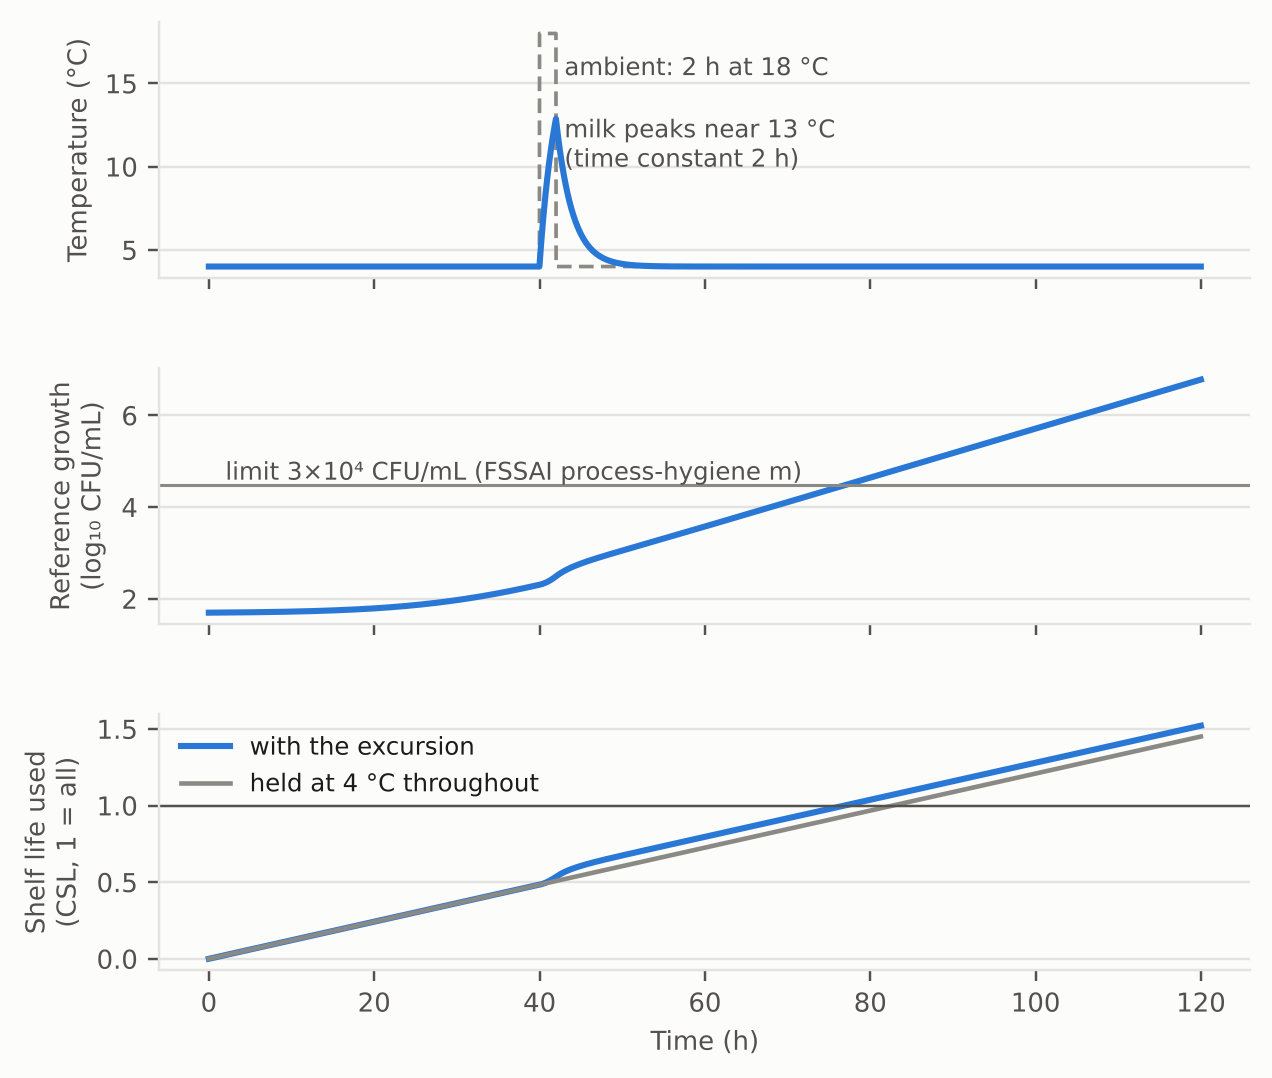
\includegraphics[width=0.86\textwidth]{trace.png}
\caption[One excursion through the models]{One excursion through the models. Top: ambient temperature (2\,h at 18\degC) and product temperature of an insulated crate. Middle: reference growth. Bottom: cumulative shelf life with and without the excursion}\label{fig:trace}\end{figure}

\section{An illustrative trip}
Figure~\ref{fig:story} shows the central difficulty on one 72-h delivery. Three cartons travel together and therefore share a single temperature history; they differ only in their starting load and the physiological state of their bacteria. The monitor, reading the log, returns one prediction for all three. It is late for one carton and early for the other two, and a more accurate thermometer cannot change that, because the information it lacks is not in the temperature record.

\begin{figure}[!htbp]\centering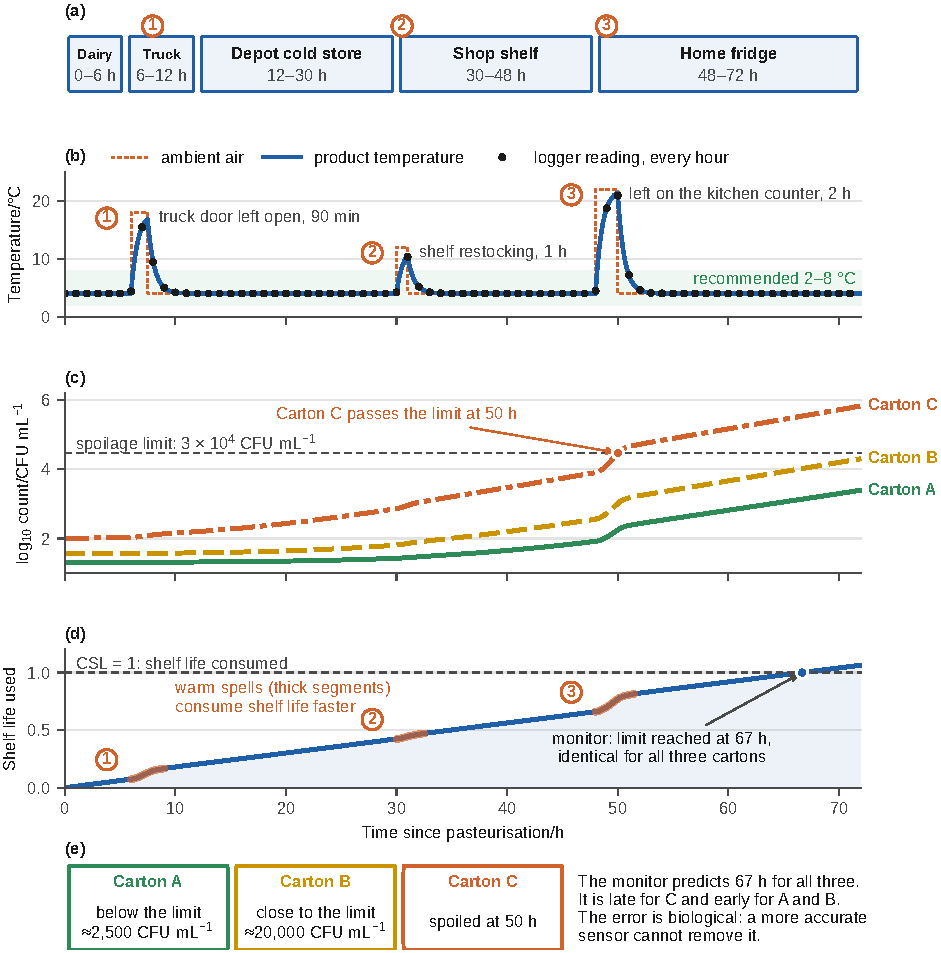
\includegraphics[width=\textwidth]{story}
\caption[One delivery, three cartons]{One delivery, three cartons. (a) Stages of the trip. (b) Ambient air and product temperature with three excursions and hourly logger readings. (c) Simulated counts in three cartons with the same history but different starting load and lag. (d) Cumulative shelf life computed by the monitor; warm spells consume shelf life faster. (e) One prediction for three cartons whose true fates differ}\label{fig:story}\end{figure}

%======================================================================
\chapter{The benchmark}\label{ch:bench}
\begin{summary}
Each simulated trip has a true temperature history and a true biology. The reference model labels it spoiled or not; the monitor sees only a sensed, sampled record. Five parameter sets, 12 settings each and 4\,000 trips per setting give 240\,000 trips, each read with every sensor, sampling rule and score.
\end{summary}
\section{Design}
Figure~\ref{fig:design} summarises the design. A simulated world supplies the truth: a temperature history, a biology and, through the reference model, a label. The monitor sees only a record that has passed through a sensor and a sampling rule, and turns it into a score. Scores are compared with labels by AUC. An oracle with the true biology and the true temperature sets the ceiling, and removing information one step at a time yields the loss budget.

\begin{figure}[!htbp]\centering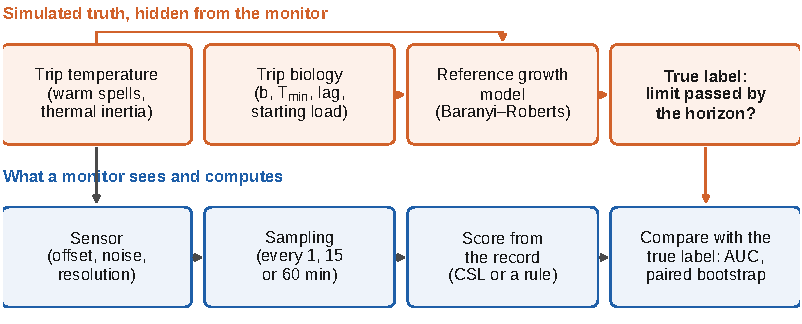
\includegraphics[width=\textwidth]{design}
\caption[Design of the benchmark]{Design of the benchmark. Top: simulated truth, hidden from the monitor. Bottom: what the monitor sees and computes. Scores are judged against the true labels by AUC}\label{fig:design}\end{figure}

\section{Trip generator}
Each trip has a product-temperature trace on a one-minute grid. The base temperature of the chain is drawn uniformly from 2.5--5\degC. Excursions arrive as a Poisson process with a mean of one per 144\,h of horizon (at most eight per trip); each peaks at 12, 14.3, 17.5 or 30.7\degC{} with weights 0.30, 0.25, 0.30 and 0.15, representing transport and retail handling, and lasts a lognormal time with median 60\,min and log-standard deviation 0.8, clipped to 10--480\,min. Product temperature follows the ambient temperature with first-order dynamics,
\begin{equation}
\frac{\dd T}{\dd t}=\frac{T_a(t)-T}{\tau_p},
\end{equation}
with the product time constant $\tau_p$ drawn from 5--20\,min for a low-mass pouch and 1--4\,h for an insulated crate. The two products form one axis of the design: in a pouch the milk follows the air closely, while in a crate a short excursion is strongly damped.

\section{Reference biology}
For each trip the reference population starts from a random load and grows by Eqs.~\eqref{eq:bar}--\eqref{eq:barq} along the trace, with
\begin{itemize}
\item $T_{\min}\sim\mathcal N(\bar T_{\min},\sigma_T^2)$, the spread between strains and trips;
\item $b=\bar b\,\varepsilon$ with $\varepsilon$ lognormal with coefficient of variation $cv\in\{0,0.10,0.25\}$;
\item $h_0$ uniform over a range derived from measured lag times;
\item $\log_{10}N_0$ uniform over an assumed range.
\end{itemize}
In the structure-risk run, a quarter of the lag state is re-imposed whenever the product temperature departs from, or returns to, its two-hour running mean by more than 4\degC, following the extra lag observed after temperature shifts \cite{zwietering1994}. The estimator is not told about this mechanism.

\section{Labels}
A trip is \emph{spoiled} if the reference population exceeds the limit within the label horizon. The horizon is the time the estimator takes to reach the limit at a constant 4\degC{} with nominal parameters, rounded up to a whole hour, as a printed shelf life would be. It was fixed from label balance before any rule was compared. Prevalence is therefore a property of the design (about 0.5 for spoilage and \NumLisPrevMin--\NumLisPrevMax{} for \textit{Listeria}), and absolute predictive values must not be read as field rates. Only ranking (AUC) and calibration against the constructed labels are interpreted.

\section{Sensors and sampling}
Each sensor adds a per-trip offset drawn uniformly within its accuracy band, white noise and quantisation:
\begin{itemize}
\item DS18B20 digital sensor: offset within $\pm0.5$\degC{} \cite{ds18b20}, noise 0.05\degC, resolution 0.0625\degC;
\item PT1000 platinum resistance sensor read by a MAX31865: offset within $\pm0.15$\degC{} (IEC 60751 Class~A \cite{iec60751}), noise 0.03\degC, resolution 0.03125\degC;
\item an ideal sensor with no error.
\end{itemize}
Sampling intervals are 1, 15 and 60\,min, plus an adaptive rule that samples every minute while the temperature is changing and every 15\,min otherwise. Every trip is read with every sensor and sampling rule, so that differences between them are measured on identical histories.

\section{Scores}
Five scores are computed from the measured record: the cumulative shelf life $\CSL$ of Eq.~\eqref{eq:csl} with nominal parameters; degree-hours above 4\degC; time above 5\degC; time above 8\degC; and the maximum temperature. The oracle computes $\CSL$ with each trip's true parameters and noise-free temperature. A sixth output, a probability, is described in \secref{sec:mc}.

\section{Parameter sets}
Table~\ref{tab:runs} lists the five runs. The baseline uses the Neumeyer parameters and a measured lag range. The extra-lag run adds the structural risk described above. The low-load run uses a starting load close to real post-pasteurisation levels. Because parameters from inoculated isolates need not describe natural flora, the milk-flora run uses parameters fitted to ComBase records of spoilage bacteria in pasteurised milk (Chapter~\ref{ch:val}). The \textit{Listeria} run models a pathogen with labels of $+0.5$ and $+1$\,log$_{10}$ growth above the starting load; these are round-number labels, not regulatory limits. Each run has 12 settings (two limits, two products, three values of $cv$) of 4\,000 trips. The full list of parameters, with the source of every value, is given in Appendix~\ref{app:params}.

\begin{table}[!htbp]
\centering\footnotesize\caption{Benchmark runs. ``Assumed'' marks values without a direct source}\label{tab:runs}
\setlength{\tabcolsep}{4pt}
\begin{tabular}{@{}p{2.2cm}p{11.8cm}@{}}\toprule\rowcolor{dghead}
Run & Biology and labels\\\midrule
Baseline & $b=0.030$, $T_{\min}=-7.7$\degC{} \cite{neumeyer1995}; $\sigma_T=1.5$\,K (assumed); $h_0\in[2.5,5]$ \cite{lin2016}; $N_0$ 30--100\,CFU\,mL$^{-1}$ (assumed); limits $3\times10^4$ and $10^6$\,CFU\,mL$^{-1}$; horizons \NumBaseHzA{} and \NumBaseHzB\,h\\
Extra lag & as baseline, plus extra lag after temperature shifts \cite{zwietering1994}\\
Low load & as baseline, $N_0$ 0.1--3\,CFU\,mL$^{-1}$ \cite{martin2021}; horizons \NumLowHzA{} and \NumLowHzB\,h\\
Milk flora & $b=\NumCbB$, $T_{\min}=\NumCbT$\degC{} (ComBase, $n=\NumCbNfit$), low load; horizons \NumCombHzA{} and \NumCombHzB\,h\\
\textit{Listeria} & $b=\NumLisB$, $T_{\min}=\NumLisT$\degC{} (ComBase, $n=\NumLisN$); $h_0\in[2,4.5]$, $\sigma_T=1.0$\,K, $N_0$ 0.06--0.18\,CFU\,mL$^{-1}$ (assumed); labels $+0.5$ and $+1$\,log; horizons \NumLisHzA{} and \NumLisHzB\,h\\\bottomrule
\end{tabular}
\end{table}

\section{Probabilistic output}\label{sec:mc}
Instead of a single verdict, the monitor can draw $M=80$ parameter sets $\theta_k=(b_k,T_{\min,k},h_{0,k},N_{0,k})$ from a prior and report
\begin{equation}\label{eq:mc}
\hat p=\frac1M\sum_{k=1}^{M}\mathbf 1\{\CSL(\theta_k)\ge1\},
\end{equation}
the fraction of plausible biologies under which the limit has been reached. Its Monte Carlo standard error is at most $\sqrt{0.25/80}=0.056$. Two priors are compared with the single alarm that uses nominal parameters: a prior that matches the simulated variation, and an overconfident prior that ignores the strain variation in $b$.

\section{Protocol}
For every run and setting: (1) generate 4\,000 temperature histories; (2) simulate the reference population and label each trip; (3) read each history with every sensor and sampling rule; (4) compute all scores and the oracle; (5) estimate every AUC with a bootstrap interval and every paired contrast with a paired-bootstrap interval; (6) compute the probability and its calibration. Random seeds are fixed, and the whole benchmark runs in about three hours on two processor cores.

%======================================================================
\chapter{Statistical methods}\label{ch:stats}
\begin{summary}
Rules are compared by AUC, which measures ranking and does not depend on the constructed prevalence. Differences between rules are tested on identical trips with a paired bootstrap, and calibration is measured by the Brier score and the expected calibration error.
\end{summary}
\section{The area under the ROC curve}
Let $S_1$ be the score of a randomly chosen spoiled trip and $S_0$ that of a randomly chosen unspoiled trip. The primary metric is
\begin{equation}\label{eq:aucdef}
\AUC=\Pr(S_1>S_0)+\tfrac12\Pr(S_1=S_0),
\end{equation}
the probability that the monitor ranks a spoiled trip above an unspoiled one \cite{hanley1982}. A value of 0.5 is a coin toss and 1 is perfect ranking. AUC does not depend on a threshold or on the prevalence, which in this benchmark is constructed, so it measures how much information a score carries. For $n_1$ spoiled and $n_0$ unspoiled trips it is estimated by the Mann--Whitney statistic \cite{mannwhitney1947},
\begin{equation}\label{eq:auc}
\widehat{\AUC}=\frac{1}{n_1n_0}\Big(\sum_{i:y_i=1}r_i-\frac{n_1(n_1+1)}{2}\Big),
\end{equation}
where $r_i$ are the ranks of the pooled scores.

\section{Precision and sample size}
Hanley and McNeil approximated the standard error of $\widehat{\AUC}$ by
\begin{equation}\label{eq:hm}
\mathrm{SE}^2=\frac{A(1-A)+(n_1-1)(Q_1-A^2)+(n_0-1)(Q_2-A^2)}{n_1n_0},
\end{equation}
with $Q_1=A/(2-A)$ and $Q_2=2A^2/(1+A)$ \cite{hanley1982}. For $A=0.67$ and $n_1=n_0=2\,000$, a typical setting, $\mathrm{SE}=0.0085$. This fixed the number of trips: the loss to biology is more than fifteen standard errors, while sensor and sampling effects are of the order of one standard error and can be resolved only by paired comparison.

\section{Bootstrap intervals}
Intervals for single AUCs are percentile intervals from $B=200$ bootstrap resamples of trips \cite{efron1993}. The trip is the resampling unit because trips are independent by construction, while the many readings within a trip are not.

\section{Paired comparisons}
Two scores computed on the same trips are correlated, because both respond to the same temperature histories. For a difference $D=\AUC_1-\AUC_2$,
\begin{equation}\label{eq:vard}
\mathrm{Var}(\hat D)=\mathrm{Var}(\widehat{\AUC}_1)+\mathrm{Var}(\widehat{\AUC}_2)-2\,\mathrm{Cov}(\widehat{\AUC}_1,\widehat{\AUC}_2),
\end{equation}
and the covariance term is large and positive for similar scores. Testing the two AUCs separately would ignore it and lose most of the power; this is why every trip is read with every sensor, sampling rule and score. The interval for $D$ is obtained by resampling the same trips for both scores $B=400$ times, the resampling counterpart of the method of DeLong et al.\ \cite{delong1988}.

\section{Multiplicity}
Each run has 12 settings and each contrast is examined in all of them. No conclusion is drawn from a single setting: for each contrast the range of the difference over the settings is reported, together with the number of settings whose 95\,\% interval excludes zero. Under no real effect about 0.3 such exclusions in a favourable direction would be expected among 12 settings by chance.

\section{Calibration}
A probability $\hat p_i$ is calibrated if, among trips given probability $p$, a fraction $p$ is spoiled. Calibration is measured by the Brier score and by the expected calibration error over ten equal-width bins \cite{brier1950,naeini2015},
\begin{gather}
\mathrm{Brier}=\frac1n\sum_i(\hat p_i-y_i)^2,\label{eq:brier}\\
\mathrm{ECE}=\sum_{m=1}^{10}\frac{|B_m|}{n}\,\big|\bar y_{B_m}-\bar p_{B_m}\big|.\label{eq:ece}
\end{gather}

\section{Growth-rate fits}
Secondary models are fitted by ordinary least squares on $\sqrt{\mu}$, with 95\,\% intervals from bootstrap resamples of records. Agreement between predicted and observed rates is summarised by the bias and accuracy factors of Ross \cite{ross1996},
\begin{equation}\label{eq:bfaf}
B_f=10^{\frac1n\sum\log_{10}(\hat\mu_i/\mu_i)},\qquad A_f=10^{\frac1n\sum|\log_{10}(\hat\mu_i/\mu_i)|},
\end{equation}
where $B_f=1$ means no bias and $A_f-1$ is the typical relative error.

%======================================================================
\chapter{Validation against real data}\label{ch:val}
\begin{summary}
The model reproduces a published fluctuating-temperature experiment within \NumLinErrAbs\,\%, fits natural spoilage flora with the same temperature shape as inoculated isolates but a lower level, and predicts held-out \textit{Listeria} growth rates without bias.
\end{summary}
\section{A fluctuating-temperature experiment}
Lin et al.\ held UHT milk inoculated with \textit{P.~fluorescens} at 4\degC, with and without two four-hour excursions to 29\degC, and report that the time to $10^6$\,CFU\,mL$^{-1}$ fell from about 90\,h to about 55\,h \cite{lin2016}. With parameters fitted only to their growth rates and their 4\degC{} lag, the reference model gives \NumLinConst\,h and \NumLinExc\,h (Fig.~\ref{fig:lin}), an error of $\NumLinErr$\,\% on the excursion case, which was not used for fitting. This is one experiment with one organism and an inoculated load far above real post-pasteurisation levels, and the published times are approximate values from the text.

\begin{figure}[!htbp]\centering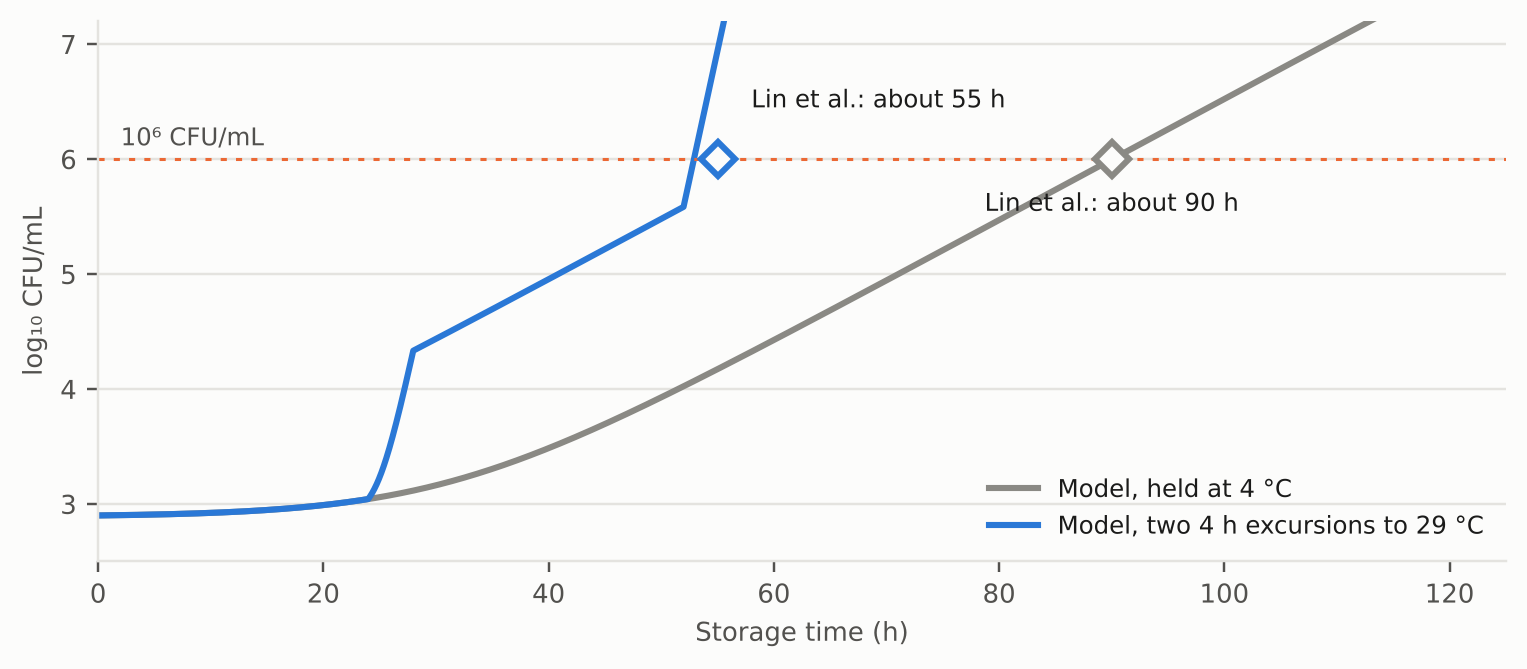
\includegraphics[width=0.66\textwidth]{lin.png}
\caption[Reproduction of a fluctuating-temperature experiment]{Reproduction of the experiment of Lin et al.\ \cite{lin2016}: model growth at a constant 4\degC{} and with two four-hour excursions to 29\degC, with the published times to $10^6$\,CFU\,mL$^{-1}$ (diamonds)}\label{fig:lin}\end{figure}

\section{Natural spoilage flora}
ComBase holds \NumCbN{} records of the maximum growth rate of aerobic spoilage bacteria in pasteurised milk at 2.7--14.9\degC{} from the Tasmanian Institute of Agriculture \cite{combase}; they are listed in Appendix~\ref{app:data}. One record at 6.8\degC{} lies far below its neighbours. Without it, the square-root law fits the remaining \NumCbNfit{} records with $b=\NumCbB$, $T_{\min}=\NumCbT$\degC{} and a residual standard deviation of \NumCbSd{} in natural-log units; with it, $b=\NumCbAllB$ and $T_{\min}=\NumCbAllT$\degC, so no conclusion depends on it. Parameters from inoculated isolates overpredict these records with a bias factor of \NumCbBias{} that is nearly constant across temperature (Fig.~\ref{fig:cb}): the temperature \emph{shape} transfers from isolates to natural flora, the \emph{level} does not. This is consistent with studies that choose a fast isolate as a worst case, and it is the reason for the milk-flora run.

\begin{figure}[!htbp]\centering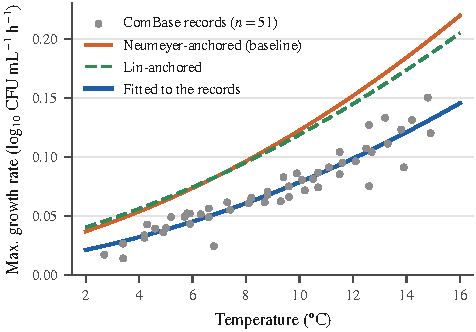
\includegraphics[width=0.66\textwidth]{combase}
\caption[Natural spoilage flora in pasteurised milk]{Maximum growth rates of natural spoilage flora in pasteurised milk (points; ComBase \cite{combase}) with the Neumeyer-anchored model (dotted), the Lin-anchored model (dashed) and the square-root fit to the records (solid)}\label{fig:cb}\end{figure}

\section{\textit{Listeria monocytogenes}}
ComBase milk records with a stated growth rate for \textit{L.~monocytogenes} at 2--16\degC{} were split by condition: \NumLisN{} records without added factors were used for fitting and \NumLisHeld{} records with other stated conditions (sterilised or previously heated milk, added salts or acids) were held out. The fit gives $b=\NumLisB$ (95\,\% bootstrap interval \NumLisBLo--\NumLisBHi) and $T_{\min}=\NumLisT$\degC{} ($\NumLisTLo$ to $\NumLisTHi$\degC), a generation time of \NumLisGen\,h at 4\degC, and on the held-out records $B_f=\NumLisBiasHeld$ and $A_f=\NumLisAccHeld$ ($A_f=\NumLisAccFit$ on the fitted records). The split is by condition rather than by study, so some held-out records share a source with fitted ones and the test is weaker than a split by source. Because $T_{\min}$ lies closer to refrigeration temperature, the rate at 13\degC{} is \NumLisRatio{} times that at 4\degC{} for \textit{Listeria}, against about 3.4 times for spoilage flora (Fig.~\ref{fig:lis}).

\begin{figure}[!htbp]\centering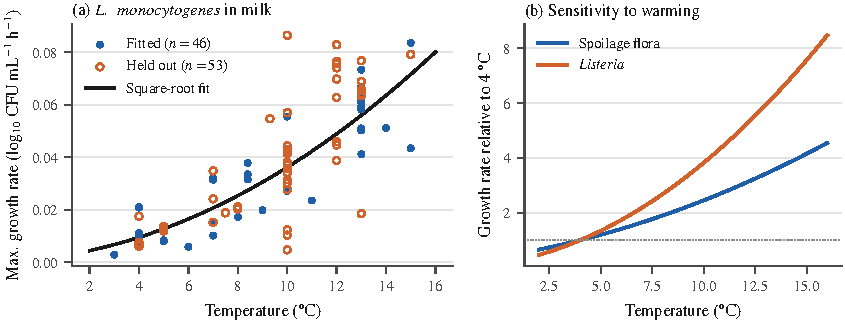
\includegraphics[width=\textwidth]{lis}
\caption[\textit{Listeria monocytogenes} in milk]{\textit{Listeria monocytogenes} in milk. (a) Maximum growth rates used for fitting (filled) and held out by condition (open), with the square-root fit (ComBase \cite{combase}). (b) Growth rate relative to 4\degC{} for spoilage flora (solid) and \textit{Listeria} (dashed)}\label{fig:lis}\end{figure}

\section{The compiled data}
A ComBase search with milk as the food matrix returned about 480 records, of which \DatNFull{} were compiled (Table~\ref{tab:dcomp}), together with the \DatNSp{} records of spoilage flora. Records without a stated rate were not used for fitting. All compiled records are released with the code.

\TabDataComp

%======================================================================
\chapter{Results}\label{ch:results}
\begin{keyresults}
\begin{itemize}[leftmargin=1.1em]
\item Unobserved biology costs \NumBaseGapMin--\NumBaseGapMax{} AUC in the baseline run, an order of magnitude more than any sensor or sampling choice.
\item A PT1000 instead of a DS18B20 gains at most \NumBaseSensMax{} AUC; hourly sampling matches one-minute sampling in \NumBaseSampNull{} of 12 settings.
\item The growth-model score beats time above 5\degC{} and the maximum temperature in every setting, but improves on degree-hours by at most \NumLagGainMax.
\item A Monte Carlo probability reaches ECE \NumBaseEceMMin--\NumBaseEceMMax; a single alarm \NumBaseEcePMin--\NumBaseEcePMax.
\item The pattern is the same in all five parameter sets.
\end{itemize}
\end{keyresults}

\section{Loss budget (RQ1)}
An oracle that knows each trip's biology and temperature separates spoiled from unspoiled trips almost perfectly, by construction. The same $\CSL$ with nominal biology and an ideal sensor loses \NumBaseGapMin--\NumBaseGapMax{} AUC across the 12 baseline settings (Table~\ref{tab:budget}, Fig.~\ref{fig:budget}). The loss is large even when strains do not differ in growth rate ($cv=0$), because the minimum growth temperature, the lag state and the starting load still differ between trips. In terms of Eq.~\eqref{eq:cslint}, these quantities set the rate scale and the budget $K$, which the temperature record does not contain; no sensor or sampling rate can recover them. Replacing the ideal sensor by a PT1000 or a DS18B20 sampled every 15 or 60\,min removes only a further 0.00--0.02.

\TabBudget

\begin{figure}[!htbp]\centering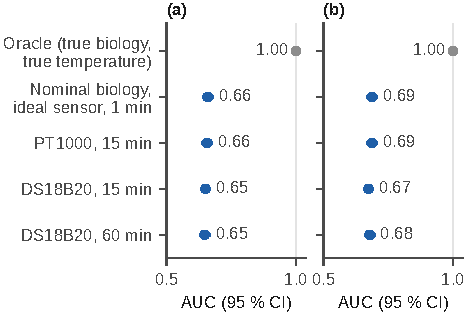
\includegraphics[width=0.66\textwidth]{budget}
\caption[Loss budget]{Loss budget for (a) a low-mass pouch and (b) an insulated crate (limit $3\times10^4$\,CFU\,mL$^{-1}$, $cv=0.10$). Grey: oracle with true biology and temperature. Blue: the growth-model score as information is removed step by step. Bars: 95\,\% bootstrap intervals}\label{fig:budget}\end{figure}

\section{Against simple rules (RQ3)}
On identical trips, the growth-model score beats time above 5\degC{} in \NumBaseFiveSig{} of 12 settings and the maximum temperature in \NumBaseMaxSig{} (Table~\ref{tab:auc}, Fig.~\ref{fig:methods}). Against degree-hours above 4\degC, a rule that needs no growth model, the gain is positive with an interval excluding zero in \NumBaseGainSig{} of 12 settings, but small: \NumBaseGainMin--\NumBaseGainMax{} AUC in the baseline run and up to \NumLagGainMax{} when extra lag is present. This is the behaviour predicted in Chapter~\ref{ch:models}: degree-hours are the linear part of the same integral, and the growth model gains only on the large excursions where the quadratic part matters. Time above 8\degC{} and the maximum temperature discard the duration or the depth of an excursion and rank trips worst.

\begin{figure}[!htbp]\centering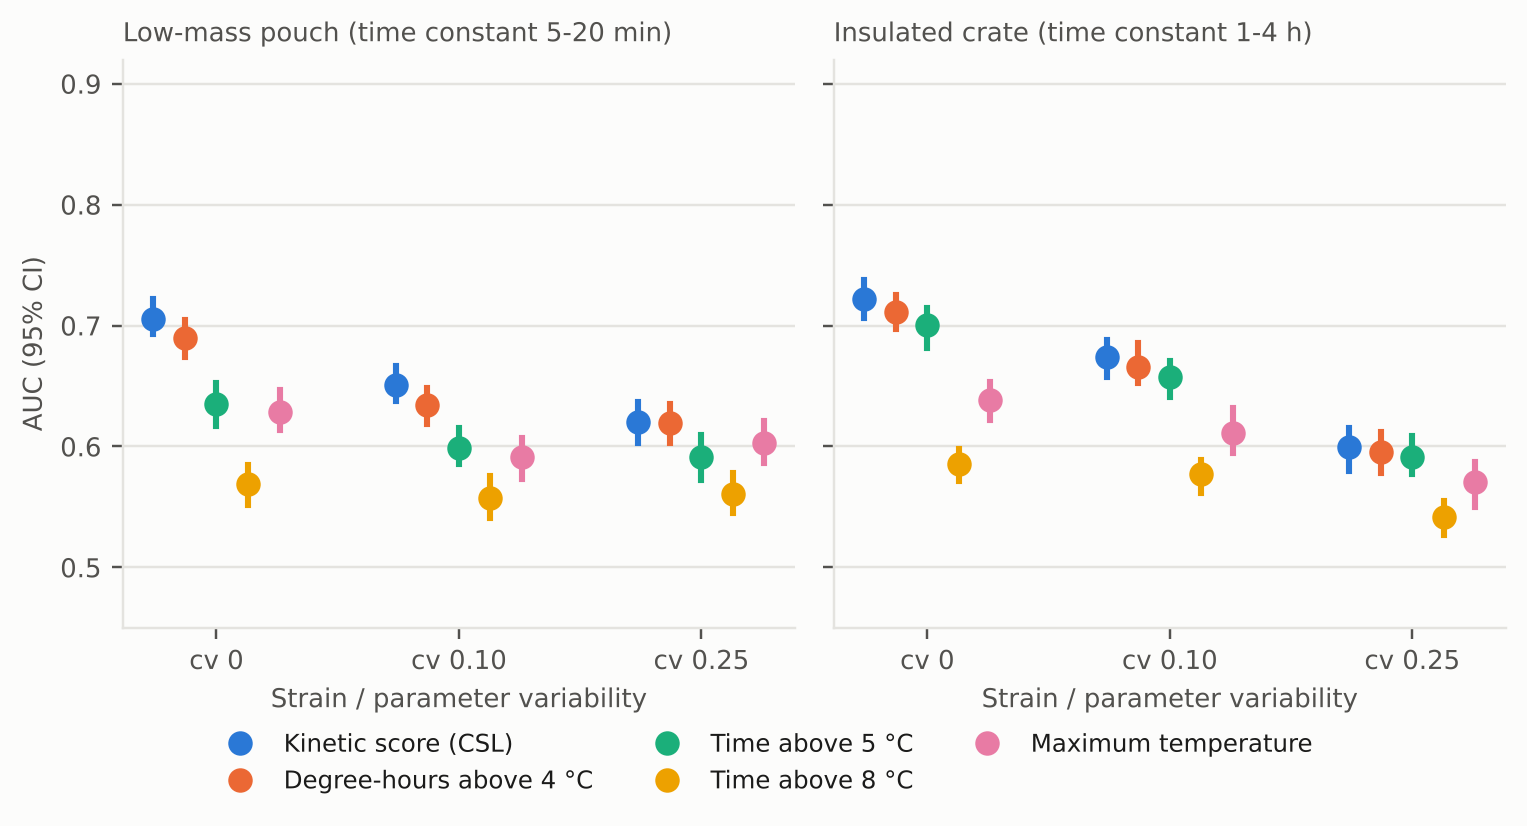
\includegraphics[width=\textwidth]{methods.png}
\caption[AUC of the five scores]{AUC of the five scores from a DS18B20 record sampled every 15\,min in the baseline run, by product and strain variability (limit $3\times10^4$\,CFU\,mL$^{-1}$). Bars: 95\,\% bootstrap intervals}\label{fig:methods}\end{figure}

{\renewcommand{\footnotesize}{\scriptsize}\TabAUC}

\section{Sensors and sampling (RQ2)}
Replacing a DS18B20 with a PT1000 gains \NumBaseSensMin--\NumBaseSensMax{} AUC at 15-min sampling (Table~\ref{tab:contrasts}, Fig.~\ref{fig:forest}). The reason is visible in Eq.~\eqref{eq:sqrt}: a sensor offset of $\pm0.5$\degC{} shifts $\sqrt{\mu}$ by $0.5b$, about 4\,\% of its value at 4\degC, whereas the trip-to-trip spread of $T_{\min}$, $h_0$ and $N_0$ moves the rate scale and the budget by tens of per cent. Sampling hourly instead of every minute shows no detectable difference in \NumBaseSampNull{} of 12 settings and at most about 0.01 where it does, and the adaptive rule is indistinguishable from fixed one-minute sampling. Excursions in the generator last at least 10\,min and typically an hour; the conclusion on sampling would change if short, sharp excursions were common.

{\renewcommand{\footnotesize}{\scriptsize}\TabContrasts}

\begin{figure}[!htbp]\centering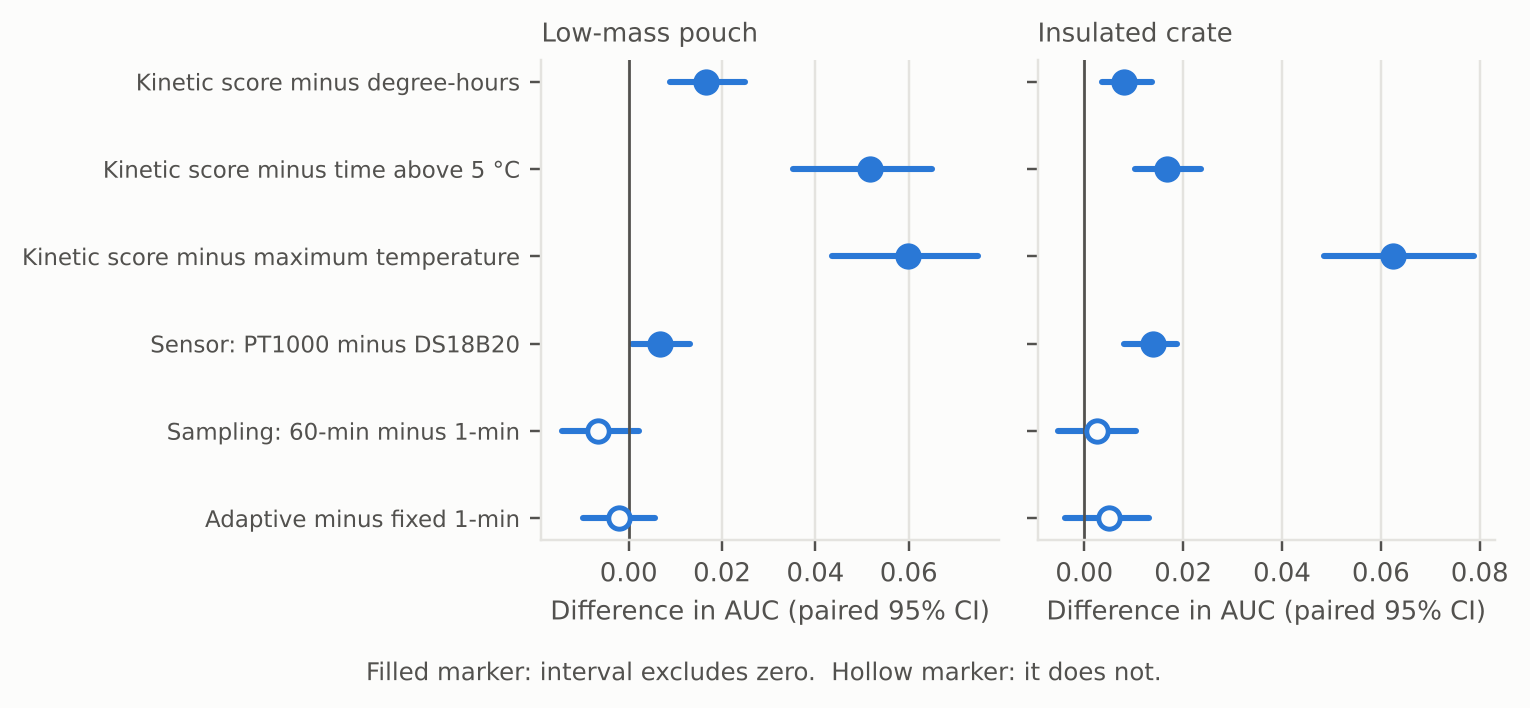
\includegraphics[width=0.92\textwidth]{forest.png}
\caption[Paired differences in the baseline run]{Paired AUC differences on identical trips in one baseline setting per product ($cv=0.10$, limit $3\times10^4$\,CFU\,mL$^{-1}$), with 95\,\% paired-bootstrap intervals. Filled markers: interval excludes zero}\label{fig:forest}\end{figure}

\section{Robustness across parameter sets}
Figure~\ref{fig:runs} summarises the four effects across all five runs. The pattern holds whether the biology is anchored to inoculated isolates, includes extra lag, starts from a realistic low load, is fitted to natural flora or describes \textit{Listeria}: the biology gap is \NumLowGapMin--\NumLowGapMax{} (low load), \NumCombGapMin--\NumCombGapMax{} (milk flora) and \NumLisGapMin--\NumLisGapMax{} (\textit{Listeria}); the gain over degree-hours stays below \NumLagGainMax{} in every run; and the sensor gain stays small.

\begin{figure}[!htbp]\centering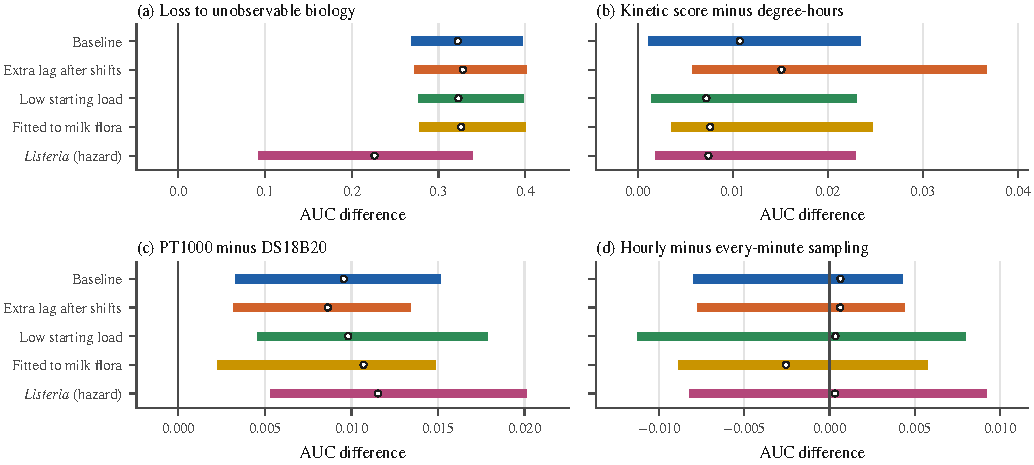
\includegraphics[width=\textwidth]{runs}
\caption[Four effects across the five parameter sets]{Four effects across the five parameter sets, as AUC differences on identical trips: (a) loss to unobserved biology, (b) growth-model score over degree-hours, (c) PT1000 over DS18B20, (d) hourly over one-minute sampling. Bars span the 12 settings of each run; dots mark the median. Horizontal scales differ}\label{fig:runs}\end{figure}

\section{Calibration (RQ4)}
A single alarm with nominal parameters is badly calibrated against the constructed labels (ECE \NumBaseEcePMin--\NumBaseEcePMax; Table~\ref{tab:cal}, Fig.~\ref{fig:cal}). A Monte Carlo probability with a prior that matches the truth reaches ECE \NumBaseEceMMin--\NumBaseEceMMax, and one with an overconfident prior on the growth rate \NumBaseEceOMin--\NumBaseEceOMax. Absolute values reflect the constructed prevalence; the ordering of the three variants is the finding. A probability that admits what the log cannot know is better calibrated than a verdict that ignores it, and even a prior that understates the strain variation retains most of the benefit.

{\renewcommand{\footnotesize}{\scriptsize}\TabCal}

\begin{figure}[!htbp]\centering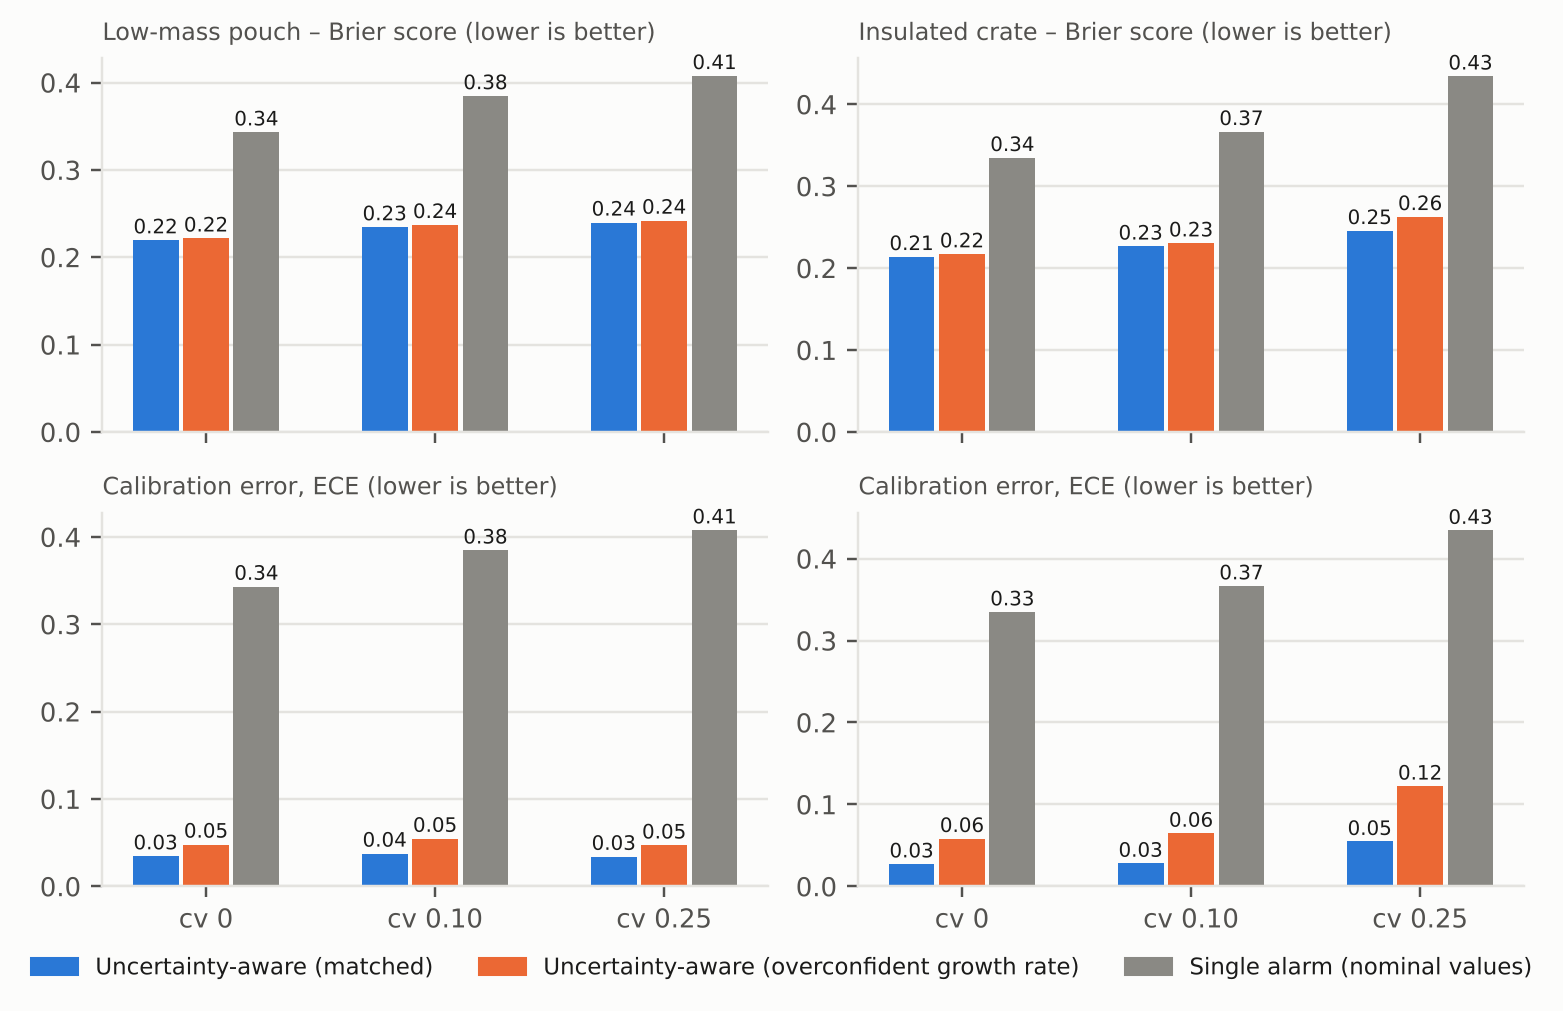
\includegraphics[width=\textwidth]{calibration.png}
\caption[Calibration of probabilities and alarms]{Brier score and expected calibration error of the Monte Carlo probability with a matched prior, with an overconfident prior, and of a single alarm with nominal parameters (baseline run, limit $3\times10^4$\,CFU\,mL$^{-1}$). Lower is better}\label{fig:cal}\end{figure}

%======================================================================
\chapter{\textit{Listeria monocytogenes}: a hazard case study}\label{ch:listeria}
\begin{summary}
For a pathogen with a minimum growth temperature close to refrigeration, a warm hour costs more, but the loss budget has the same shape: biology first, instruments a distant second.
\end{summary}
\section{Why a pathogen behaves differently}
The \textit{Listeria} fit places $T_{\min}$ at \NumLisT\degC, much closer to refrigeration than the $-7.7$\degC{} of spoilage \textit{Pseudomonas}. By Eq.~\eqref{eq:ratio}, the same warm hour is therefore relatively more expensive: the rate at 13\degC{} is \NumLisRatio{} times the rate at 4\degC, against about three times for spoilage flora. At 4\degC{} itself growth is slow, with a generation time of \NumLisGen\,h. Temperature excursions thus matter even more for the hazard than for spoilage.

\section{Results}
With labels of $+0.5$ and $+1$\,log$_{10}$ growth, unobserved biology costs \NumLisGapMin--\NumLisGapMax{} AUC, a PT1000 gains \NumLisSensMin--\NumLisSensMax, hourly sampling matches minute sampling in \NumLisSampNull{} of 12 settings, and the gain of the growth-model score over degree-hours is at most \NumLisGainMax{} (Tables~\ref{tab:budget}--\ref{tab:cal}). The lower end of the biology gap is smaller than for spoilage because the narrow starting-load range and the slow growth at 4\degC{} leave less room for biological differences to reorder trips.

\section{Labels and estimator structure}
The half-log label requires a caveat. The limit then lies inside the lag-to-growth transition, where the Gompertz estimator approximates the Baranyi--Roberts reference poorly; even the oracle reaches only \NumLisOrcAMin--\NumLisOrcAMax{} AUC (\NumLisOrcBMin--\NumLisOrcBMax{} for the $+1$\,log label). With the $+1$\,log label the probability reaches ECE \NumLisEceBMMin--\NumLisEceBMMax{} against \NumLisEceBPMin--\NumLisEceBPMax{} for the alarm; with the half-log label it remains better than the alarm (\NumLisEceAMMin--\NumLisEceAMMax{} against \NumLisEceAPMin--\NumLisEceAPMax) but is poorly calibrated in absolute terms. For very small growth targets, the structure of the estimator, and not biology alone, limits accuracy.

\section{Scope}
This case study concerns growth, not illness. Risk of illness depends on dose, virulence, host susceptibility and the contamination event, none of which are modelled. The FSSAI criterion for \textit{L.~monocytogenes} in milk products is absence in 25\,mL \cite{fssai2024}, which no growth threshold represents.

%======================================================================
\chapter{Monitor design and software}\label{ch:design}
\begin{summary}
The results translate into a short list of design rules. The estimator runs on a microcontroller, a browser demonstrator runs the same kernel, and the whole study is reproducible from one command.
\end{summary}
\section{Design rules}
Table~\ref{tab:rules} converts the results into rules for a milk cold-chain monitor.

\begin{table}[!htbp]\centering\footnotesize
\caption{Design rules for a milk cold-chain monitor}\label{tab:rules}
\begin{tabular}{@{}p{2.6cm}p{11.2cm}@{}}\toprule\rowcolor{dghead}
Decision & Rule and evidence\\\midrule
Sensor & A $\pm0.5$\degC{} digital probe suffices; a PT1000 gains at most \NumBaseSensMax{} AUC\\
Sampling & 15--60\,min is enough unless excursions shorter than about 10\,min are common\\
Score & Cumulative shelf life; degree-hours above 4\degC{} are an acceptable fallback (at most \NumLagGainMax{} AUC lower)\\
Rules to avoid & Maximum temperature and time above 8\degC; both rank trips clearly worse\\
Output & A probability, not an alarm (ECE \NumBaseEceMMin--\NumBaseEceMMax{} against \NumBaseEcePMin--\NumBaseEcePMax)\\
Parameters & Fit to natural flora of the product; inoculated isolates overpredict by a factor of \NumCbBias\\
Improvement & Measure the biology: starting load, lag and strain spread\\
\bottomrule\end{tabular}\end{table}

\section{Processing on the logger}
Figure~\ref{fig:system} shows how the estimator runs on a logger. A probe reading is taken on an adaptive schedule, the shelf-life rate $1/\SL(T)$ is read from a stored table, Eq.~\eqref{eq:csl} is updated, and the same sum is carried for 80 sampled biological parameter sets to produce a probability. Parameter fitting and the shelf-life table are prepared once, offline. The memory required is a table of a few thousand entries and 80 running sums, well within a low-cost microcontroller.

\begin{figure}[!htbp]\centering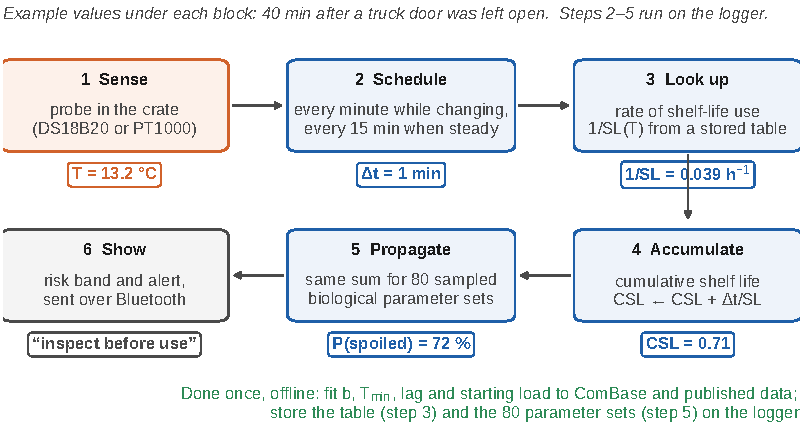
\includegraphics[width=\textwidth]{system}
\caption[Processing on the logger]{Processing on the logger, with example values 40\,min after a truck door was left open. Steps 2--5 run on the device; parameter fitting and the shelf-life table are prepared offline}\label{fig:system}\end{figure}

\section{Software}
The repository is organised in layers. A kinetics module implements Eqs.~\eqref{eq:sqrt}--\eqref{eq:csl}; a simulator implements Chapter~\ref{ch:bench}; the benchmark computes scores, AUCs, paired bootstraps and calibration; validation scripts reproduce Chapter~\ref{ch:val}; and scripts write every number, table and figure of the paper and of this monograph from the result files. Numerical work uses NumPy, SciPy and Matplotlib \cite{harris2020,virtanen2020,hunter2007}. Fourteen automated tests (Table~\ref{tab:tests}) run on every change. Parts of the simulation code were developed with an AI coding assistant; all of it is covered by the tests and was checked by the author.

\begin{table}[!htbp]\centering\footnotesize
\caption{Automated tests}\label{tab:tests}
\begin{tabular}{@{}p{2.6cm}p{11.2cm}@{}}\toprule\rowcolor{dghead}
Group & What is checked\\\midrule
Kinetics (4) & Gompertz agrees with exponential growth; reference and estimator agree at constant temperature with equal parameters; the look-up table matches the closed form; shelf life falls with temperature\\
Validation (3) & Fitted parameters are plausible; the constant-4\degC{} and two-excursion times of Lin et al.\ are reproduced within 10\,\%\\
Statistics (6) & Fast AUC matches a reference implementation; known AUC values are recovered; the paired difference of identical scores is zero; a real improvement is detected; the probability rises with temperature; calibration of perfect and poor forecasts\\
Parity (1) & The browser kernel matches the Python kernel\\
\bottomrule\end{tabular}\end{table}

\section{Browser demonstrator}
A public demonstrator runs the same kernel in the browser (\url{https://copyninja07-07.github.io/dairyguard/explorer.html}); a parity test ensures that it reproduces the Python implementation. A user chooses or draws a trip, such as a shop door left open or a failed truck refrigerator, and sees the probability that the milk has passed the limit, the simulated fate of 60 cartons and the comparison with a single alarm. The demonstrator is software only; a hardware logger is future work.

%======================================================================
\chapter{Discussion}\label{ch:disc}
\section{Where effort belongs}
In every run, what the thermometer cannot observe costs about an order of magnitude more accuracy than any choice of sensor or sampling interval. Equation~\eqref{eq:cslint} explains why: a log measures the integral of the growth rate well, but the rate scale and the budget against which the integral is compared vary from carton to carton. A more accurate thermometer is therefore a poor way to improve a spoilage estimate, and a low-cost probe sampled every 15--60\,min loses little under the assumptions made here. Effort is better spent on the biology: measuring the starting load or a proxy of handling history, learning the lag and strain spread of the product at hand, and reporting a probability instead of a verdict.

\section{Consistency with earlier studies}
Sensitivity analyses of milk spoilage rank storage temperature among the most influential inputs \cite{lau2022,buehler2018,qian2023,giannakourou2020}; this study finds that biology dominates. The two answer different questions. When temperature is drawn from a distribution, it drives the spread of outcomes; once it is measured, the residual uncertainty is biological. The small gain of the growth-model score over degree-hours agrees with the long practical use of degree-hour and time--temperature integrators \cite{taoukis1989,kim2020}, and the finding that parameters from inoculated isolates overpredict natural flora agrees with the practice of choosing a fast isolate as a worst case.

\section{Hazard and spoilage}
For spoilage flora a warm hour is costly but the baseline rate is already high; for \textit{Listeria}, growth at 4\degC{} is slow but rises about \NumLisRatio-fold by 13\degC. The same benchmark and the same design rules hold for both, which supports treating temperature excursions as the common risk factor while recognising that a growth model says nothing about illness.

\section{Limitations}
\begin{enumerate}[label=(\roman*)]
\item The reference and the estimator both reduce the temperature history to an integral of the growth rate, so the benchmark measures how much accuracy is lost to the listed sources, not whether a growth-model score describes growth better than another model; the structure-risk run relaxes one structural assumption only.
\item The strain spread, the starting load, the excursion statistics and the \textit{Listeria} lag are assumed (Appendix~\ref{app:params}).
\item Labels are constructed, with prevalence near 0.5 for spoilage and \NumLisPrevMin--\NumLisPrevMax{} for \textit{Listeria}.
\item ComBase records come from heterogeneous studies and report maximum rates, not curves, so lag and responses to temperature shifts are untested on them.
\item A single experiment validates growth under fluctuating temperature, and no new plate counts were made.
\item Neither organism class represents spore-formers, which account for a large share of milk spoilage \cite{martin2021}.
\item For very small growth targets, such as the half-log \textit{Listeria} label, the estimator's structure rather than biology limits accuracy.
\end{enumerate}

%======================================================================
\chapter{Conclusions}\label{ch:concl}
A temperature log can say much about how much growth the milk \emph{could} have had, and little about how much it \emph{did}. In an open benchmark of 240\,000 trips anchored to published and ComBase data, unobserved biology costs \NumBaseGapMin--\NumBaseGapMax{} AUC; a degree-hour count comes within \NumLagGainMax{} of a growth model; sensor quality and sampling interval matter little; and a Monte Carlo probability is far better calibrated than an alarm. The answers to the four research questions are therefore:
\begin{enumerate}[label=RQ\arabic*.,leftmargin=3em]
\item Biology the log cannot see is the dominant loss in every run.
\item A better sensor or faster sampling recovers at most about 0.02 AUC.
\item A growth-model score clearly beats threshold and maximum rules but only narrowly beats degree-hours.
\item A probability is far better calibrated than a single alarm.
\end{enumerate}
Four directions follow: measurements of real logger data from Indian dairy routes to replace the assumed excursion model; challenge tests with natural flora under fluctuating temperature, with new plate counts; methods that measure the biology of a lot cheaply at dispatch; and a hardware logger running the estimator. An extended study, which develops the kinetic theory behind these findings, is in preparation.

\section*{Acknowledgements}
The author thanks Dr.\ Neeraj Tripathi (School of Electronics and Communication Engineering, Shri Mata Vaishno Devi University) for guidance, and the ComBase consortium and the laboratories whose published growth records made this study possible.

%======================================================================
\appendix
\chapter{Parameters and provenance}\label{app:params}
Every parameter of the simulation is listed in Table~\ref{tab:params} with its value and its source. Values marked as assumed are the main candidates for measurement.

\TabParams

\chapter{Data}\label{app:data}
Table~\ref{tab:dsp} lists the ComBase records of spoilage flora used in Chapter~\ref{ch:val}. The complete compilation of \DatNFull{} milk records, including the \DatNLis{} \textit{Listeria} records with their conditions and sources, is in the repository (\texttt{data/combase\_milk\_records.csv}).

\TabSpRecords

\chapter{Reproducing the results}\label{app:repro}
All results are generated from fixed random seeds. With Python 3.10 or later, the packages in \texttt{requirements.txt} and a LaTeX installation:
\begin{center}\begin{tabular}{@{}ll@{}}\toprule\rowcolor{dghead}
Command & Effect\\\midrule
\texttt{make test} & run the 14 automated tests\\
\texttt{make runs} & run the five benchmark runs (about three hours on two cores)\\
\texttt{make validate} & reproduce the validation of Chapter~\ref{ch:val}\\
\texttt{make paper} & write all numbers, tables and figures and build the paper\\
\texttt{make book} & build this monograph\\
\texttt{make all} & everything above\\
\bottomrule\end{tabular}\end{center}
Every number quoted in the text is read from the result files by a script and written into the document as a macro; none is typed by hand.

\backmatter
\renewcommand{\bibname}{References}
\addcontentsline{toc}{chapter}{References}
{\small
\begin{thebibliography}{99}
\setlength{\itemsep}{1pt}
\bibitem{perez2013} Pérez-Rodríguez F, Valero A. Predictive microbiology in foods. New York: Springer; 2013. \url{https://doi.org/10.1007/978-1-4614-5520-2}
\bibitem{tarlak2023} Tarlak F. The use of predictive microbiology for the prediction of the shelf life of food products. Foods. 2023;12:4461. \url{https://doi.org/10.3390/foods12244461}
\bibitem{stavropoulou2019} Stavropoulou E, Bezirtzoglou E. Predictive modeling of microbial behavior in food. Foods. 2019;8:654. \url{https://doi.org/10.3390/foods8120654}
\bibitem{badiamelis2018} Badia-Melis R, Mc Carthy U, Ruiz-Garcia L, Garcia-Hierro J, Robla Villalba JI. New trends in cold chain monitoring applications -- a review. Food Control. 2018;86:170--82. \url{https://doi.org/10.1016/j.foodcont.2017.11.022}
\bibitem{mercier2017} Mercier S, Villeneuve S, Mondor M, Uysal I. Time--temperature management along the food cold chain: a review of recent developments. Compr Rev Food Sci Food Saf. 2017;16:647--67. \url{https://doi.org/10.1111/1541-4337.12269}
\bibitem{jedermann2014} Jedermann R, Nicometo M, Uysal I, et al. Reducing food losses by intelligent food logistics. Philos Trans R Soc A. 2014;372:20130302. \url{https://doi.org/10.1098/rsta.2013.0302}
\bibitem{koutsoumanis2005} Koutsoumanis K, Taoukis PS, Nychas G-JE. Development of a Safety Monitoring and Assurance System for chilled food products. Int J Food Microbiol. 2005;100:253--60. \url{https://doi.org/10.1016/j.ijfoodmicro.2004.10.024}
\bibitem{goransson2018} Göransson M, Nilsson F, Jevinger Å. Temperature performance and food shelf-life accuracy in cold food supply chains: insights from multiple field studies. Food Control. 2018;86:332--41. \url{https://www.sciencedirect.com/science/article/pii/S0956713517305145}
\bibitem{kim2020} Kim J, Santos CA, Kim B-S, Kim J, Koo J. Estimation of real-time remaining shelf life using mean kinetic temperature. LWT. 2020;134:109968. \url{https://doi.org/10.1016/j.lwt.2020.109968}
\bibitem{martin2021} Martin NH, Torres-Frenzel P, Wiedmann M. Invited review: controlling dairy product spoilage to reduce food loss and waste. J Dairy Sci. 2021;104:1251--61. \url{https://doi.org/10.3168/jds.2020-19130}
\bibitem{ranieri2009} Ranieri ML, Boor KJ. Short communication: bacterial ecology of high-temperature, short-time pasteurized milk processed in the United States. J Dairy Sci. 2009;92:4833--40. \url{https://doi.org/10.3168/jds.2009-2181}
\bibitem{who2015} World Health Organization. WHO's first ever global estimates of foodborne diseases find children under 5 account for almost one third of deaths. News release, 3 December 2015. \url{https://www.who.int/news/item/03-12-2015-who-s-first-ever-global-estimates-of-foodborne-diseases-find-children-under-5-account-for-almost-one-third-of-deaths}
\bibitem{fssai2024} Food Safety and Standards Authority of India. Appendix B: microbiological requirements, version 2 (4 November 2024), Tables 2A and 2B. \url{https://fssai.gov.in/upload/uploadfiles/files/Appendix%20B(1).pdf}
\bibitem{lin2016} Lin H, Shavezipur M, Yousef A, Maleky F. Prediction of growth of \textit{Pseudomonas fluorescens} in milk during storage under fluctuating temperature. J Dairy Sci. 2016;99:1822--30. \url{https://doi.org/10.3168/jds.2015-10179}
\bibitem{lima2026} Lima L, Pereira AI, Pintado M, Carocho M. Fresh dairy quality in the era of smart food systems: deterioration pathways, analytical technologies, and predictive modeling. Foods. 2026;15:3439. \url{https://doi.org/10.3390/foods15193439}
\bibitem{gompertz1825} Gompertz B. On the nature of the function expressive of the law of human mortality, and on a new mode of determining the value of life contingencies. Philos Trans R Soc Lond. 1825;115:513--83. \url{https://doi.org/10.1098/rstl.1825.0026}
\bibitem{zwietering1990} Zwietering MH, Jongenburger I, Rombouts FM, van 't Riet K. Modeling of the bacterial growth curve. Appl Environ Microbiol. 1990;56:1875--81. \url{https://doi.org/10.1128/aem.56.6.1875-1881.1990}
\bibitem{baranyi1993} Baranyi J, Roberts TA, McClure P. A non-autonomous differential equation to model bacterial growth. Food Microbiol. 1993;10:43--59. \url{https://doi.org/10.1006/fmic.1993.1005}
\bibitem{baranyi1994} Baranyi J, Roberts TA. A dynamic approach to predicting bacterial growth in food. Int J Food Microbiol. 1994;23:277--94. \url{https://doi.org/10.1016/0168-1605(94)90157-0}
\bibitem{ratkowsky1982} Ratkowsky DA, Olley J, McMeekin TA, Ball A. Relationship between temperature and growth rate of bacterial cultures. J Bacteriol. 1982;149:1--5. \url{https://doi.org/10.1128/jb.149.1.1-5.1982}
\bibitem{rosso1993} Rosso L, Lobry JR, Flandrois JP. An unexpected correlation between cardinal temperatures of microbial growth highlighted by a new model. J Theor Biol. 1993;162:447--63. \url{https://doi.org/10.1006/jtbi.1993.1099}
\bibitem{taoukis1989} Taoukis PS, Labuza TP. Applicability of time-temperature indicators as shelf life monitors of food products. J Food Sci. 1989;54:783--8. \url{https://doi.org/10.1111/j.1365-2621.1989.tb07882.x}
\bibitem{baranyi2004} Baranyi J, Tamplin ML. ComBase: a common database on microbial responses to food environments. J Food Prot. 2004;67:1967--71. \url{https://doi.org/10.4315/0362-028X-67.9.1967}
\bibitem{combase} ComBase. Database of microbial responses to food environments: growth records with milk as the food matrix. Accessed 19 Oct 2026. \url{https://www.combase.cc}
\bibitem{neumeyer1995} Neumeyer K. Modelling pseudomonad growth in milk and milk-based products. Research Master thesis. Hobart: University of Tasmania; 1995. \url{https://eprints.utas.edu.au/21013/}
\bibitem{neumeyer1997a} Neumeyer K, Ross T, McMeekin TA. Development of a predictive model to describe the effects of temperature and water activity on the growth of spoilage pseudomonads. Int J Food Microbiol. 1997;38:45--54. \url{https://doi.org/10.1016/S0168-1605(97)00089-5}
\bibitem{corradini2005} Corradini MG, Peleg M. Estimating non-isothermal bacterial growth in foods from isothermal experimental data. J Appl Microbiol. 2005;99:187--200. \url{https://doi.org/10.1111/j.1365-2672.2005.02570.x}
\bibitem{zwietering1994} Zwietering MH, de Wit JC, Cuppers HGAM, van 't Riet K. Modeling of bacterial growth with shifts in temperature. Appl Environ Microbiol. 1994;60:204--13. \url{https://doi.org/10.1128/aem.60.1.204-213.1994}
\bibitem{koutsoumanis2001} Koutsoumanis K. Predictive modeling of the shelf life of fish under nonisothermal conditions. Appl Environ Microbiol. 2001;67:1821--9. \url{https://doi.org/10.1128/AEM.67.4.1821-1829.2001}
\bibitem{ndraha2018} Ndraha N, Hsiao H-I, Vlajic J, Yang M-F, Lin H-TV. Time-temperature abuse in the food cold chain: review of issues, challenges, and recommendations. Food Control. 2018;89:12--21. \url{https://doi.org/10.1016/j.foodcont.2018.01.027}
\bibitem{zou2023} Zou Y, Wu J, Wang X, Morales K, Liu G, Manzardo A. An improved artificial neural network using multi-source data to estimate food temperature during multi-temperature delivery. J Food Eng. 2023;351:111518. \url{https://doi.org/10.1016/j.jfoodeng.2023.111518}
\bibitem{muller2026} Müller WA, Kronbauer M, Ferreira SB, da Silva SB. Computational assessment of temperature failures in the cold supply chain: implications for beef shelf life. Food Control. 2026;187:112100. \url{https://doi.org/10.1016/j.foodcont.2026.112100}
\bibitem{sofat2026} Sofat A, Sodhi B. Beyond thresholds: a quality-aware decision intelligence framework for cold chain IoT systems. arXiv preprint arXiv:2608.15082. 2026. \url{https://arxiv.org/abs/2608.15082}
\bibitem{nauta2000} Nauta MJ. Separation of uncertainty and variability in quantitative microbial risk assessment models. Int J Food Microbiol. 2000;57:9--18. \url{https://doi.org/10.1016/S0168-1605(00)00225-7}
\bibitem{lau2022} Lau S, Trmčić A, Martin NH, Wiedmann M, Murphy SI. Development of a Monte Carlo simulation model to predict pasteurized fluid milk spoilage due to post-pasteurization contamination with gram-negative bacteria. J Dairy Sci. 2022;105:1978--98. \url{https://doi.org/10.3168/jds.2021-21316}
\bibitem{buehler2018} Buehler AJ, Martin NH, Boor KJ, Wiedmann M. Psychrotolerant spore-former growth characterization for the development of a dairy spoilage predictive model. J Dairy Sci. 2018;101:6964--81. \url{https://doi.org/10.3168/jds.2018-14501}
\bibitem{qian2023} Qian C, Murphy SI, Lott TT, Martin NH, Wiedmann M. Development and deployment of a supply-chain digital tool to predict fluid-milk spoilage due to psychrotolerant sporeformers. J Dairy Sci. 2023;106:8414--33. \url{https://doi.org/10.3168/jds.2023-23673}
\bibitem{giannakourou2020} Giannakourou MC, Taoukis PS. Holistic approach to the uncertainty in shelf life prediction of frozen foods at dynamic cold chain conditions. Foods. 2020;9:714. \url{https://doi.org/10.3390/foods9060714}
\bibitem{ds18b20} Analog Devices (Maxim Integrated). DS18B20 programmable resolution 1-Wire digital thermometer. Product page and datasheet. \url{https://www.analog.com/en/DS18B20}
\bibitem{iec60751} International Electrotechnical Commission. IEC 60751:2022 Industrial platinum resistance thermometers and platinum temperature sensors. Geneva: IEC; 2022. \url{https://webstore.iec.ch/en/publication/63753}
\bibitem{hanley1982} Hanley JA, McNeil BJ. The meaning and use of the area under a receiver operating characteristic (ROC) curve. Radiology. 1982;143:29--36. \url{https://doi.org/10.1148/radiology.143.1.7063747}
\bibitem{mannwhitney1947} Mann HB, Whitney DR. On a test of whether one of two random variables is stochastically larger than the other. Ann Math Stat. 1947;18:50--60. \url{https://doi.org/10.1214/aoms/1177730491}
\bibitem{efron1993} Efron B, Tibshirani RJ. An introduction to the bootstrap. New York: Chapman \& Hall; 1993. \url{https://doi.org/10.1201/9780429246593}
\bibitem{delong1988} DeLong ER, DeLong DM, Clarke-Pearson DL. Comparing the areas under two or more correlated receiver operating characteristic curves: a nonparametric approach. Biometrics. 1988;44:837--45. \url{https://doi.org/10.2307/2531595}
\bibitem{brier1950} Brier GW. Verification of forecasts expressed in terms of probability. Mon Weather Rev. 1950;78:1--3. \url{https://doi.org/10.1175/1520-0493(1950)078<0001:VOFEIT>2.0.CO;2}
\bibitem{naeini2015} Naeini MP, Cooper GF, Hauskrecht M. Obtaining well calibrated probabilities using Bayesian binning. Proc AAAI Conf Artif Intell. 2015;29:2901--7. \url{https://doi.org/10.1609/aaai.v29i1.9602}
\bibitem{ross1996} Ross T. Indices for performance evaluation of predictive models in food microbiology. J Appl Bacteriol. 1996;81:501--8. \url{https://doi.org/10.1111/j.1365-2672.1996.tb03539.x}
\bibitem{harris2020} Harris CR, Millman KJ, van der Walt SJ, et al. Array programming with NumPy. Nature. 2020;585:357--62. \url{https://doi.org/10.1038/s41586-020-2649-2}
\bibitem{virtanen2020} Virtanen P, Gommers R, Oliphant TE, et al. SciPy 1.0: fundamental algorithms for scientific computing in Python. Nat Methods. 2020;17:261--72. \url{https://doi.org/10.1038/s41592-019-0686-2}
\bibitem{hunter2007} Hunter JD. Matplotlib: a 2D graphics environment. Comput Sci Eng. 2007;9:90--5. \url{https://doi.org/10.1109/MCSE.2007.55}

\end{thebibliography}}
\end{document}
